\chapter{Integrales de trayectoria en espacios curvos.}


	   	
\section{Teoría clásica de campos en espacios curvos.}
Al nivel más fundamental la situación que nos presenta la fisica teórica es un modelo, con un alto grado de soporte experimental, en el cual solo hay tres interacciones: la cromo-dinámica cuaántica (QCD), que explica la interacción mediante la cual los quarks interactúan para formar los hadrones; la interacción débil (EW) que explica los procesos de decaimiento radiactivo y los fenomenos electromagneticos en una teoría unificada; y finalmente la gravedad. Las primeras dos interacciones se entienden en el contexto de la teoria cuántica de campos, en particular la teoría de campos Gauge, donde las interacciones se explican mediante el intercambio de bosones Gauge (gluones para QCD y el fotón y los bosones W,Z para EW). Sin embargo la teoría que mejor explica los fenómenos gravitatorios. la relativdad general (GR), es una teoría totalmente diferente debido a su naturaleza geométrica.
\\
\\
Sin embargo el objetivo de la física es reducir el numero de teorías, conceptos y esquemas al mínimo, es por esto que muchos físicos trabajan en teorías que unifiquen estos dos esquemas: supergravedad, teoría de supercuerdas, gravedad cuántica de lazos, etc. Debido a que las otras dos interacciones fundamentales se entienden en términos de teorías cuánticas de campo, ¿no deberia darsele a la gravedad un tratamiento cuántico?
\\
Por tanto, en una busqueda de teorías más alla de GR, ¿hacia dónde nos dirigimos?. Es bien sabido que no se puede hacer con las otras fuerzas fundamentales lo mismo que con la gravedad, en la teoría gravitatoria uno cambia la aceleración producida por la fuerza gravitacional por un sistema de referencia acelerado y esto se puede hacer debido a la equivalencia entre masa inercial y masa gravitatoria. Sin embargo esto no se puede hacer con las fuerzas fundamentales restantes, por ejemplo, la aceleración que sufre una partícula cargada electricamente es proporcional a su carga e inversamente proporcional a su masa inercial ($a\propto \frac{q}{m}$). Como esta razón no es la misma para todas las partículas uno no puede encontrar un sistema de referencia donde globalmente "desaparezca" la fuerza eléctrica. Sin embargo en los 60`s se dieron cuenta que al \textit{calibrar} (traducción del ingles "gauging", refiríendose a transformaciones Gauge como transformaciones de calibre) la simetría de Lorentz, uno termina con una teoría muy parecida a la GR. En esta primera sección introduciremos esta idea, sin embargo antes daremos un ejemplo de teorías Gauge abelianas (electromagnetismo) y no-abelianas (campos de Yang Mills).
\subsection{Caso abeliano.}
Consideremeos un campo escalar complejo que obedece la ecuacion de K-G y tiene una densidad Lagrangiana:
\begin{equation}
\mathcal{L}=\partial_{\mu}\phi\partial^{\mu}\phi^{*}+m^{2}\phi\phi^{*}.
\end{equation}
Esta densidad lagrangiana posee una simetría bago $\phi\to e^{-i\Lambda}\phi,\ \ \phi^{*}\to e^{i\Lambda}\phi^{*}$ donde $\Lambda$ es un parámetro constante, vemos que esta transformación deja a $\mathcal{L}$ invariante es decir $\delta\mathcal{L}=0$. Esta transformación es llamada transformación Gauge del primer tipo. En la versión infinitesimal de la transformación tenemos:
\begin{equation}
\delta\phi=-i\Lambda\phi,\ \ \delta\phi^{*}=i\Lambda\phi^{*},\ \ \delta(\partial_{\mu}\phi)=-i\Lambda\partial_{\mu}\phi,\ \ \delta(\partial_{\mu}\phi^{*})=i\Lambda\partial_{\mu}\phi^{*},
\end{equation}
con esto definimos la corriente $j^{\mu}$ como:
\begin{eqnarray}
\nonumber \Lambda j^{\mu}&=&\frac{\partial\mathcal{L}}{\partial(\partial_{\mu}\phi)}(\delta\phi)+\frac{\partial\mathcal{L}}{\partial(\partial_{\mu}\phi^{*})}(\delta\phi^{*})=(\partial_{\mu}\phi^{*})(-i\Lambda\phi)+(\partial_{\mu}\phi)(i\Lambda\phi^{*})\\
j^\mu &=& i((\partial_{\mu}\phi)\phi^{*}-\phi(\partial_{\mu}\phi^{*})),
\end{eqnarray}
de donde
\begin{eqnarray}
\partial_\mu j^\mu &=& 0\\
\partial_{0}j^{0}=\partial_{i}j^{i}&\Rightarrow &\partial_{0}\int_{V}j^{0}dV=\int_{V}\nabla\cdot\vec{j}dV=\int_{\partial V}\vec{n}\cdot\vec{j}dS=0,
\end{eqnarray} 
por tanto
\begin{equation}
\partial_{0}\int_{V}j^{0}dV=0\Rightarrow\frac{dQ}{dt}=0;\ \ Q=\int_{V}j^{0}dV.
\end{equation}
Identificando $Q$ con la carga eléctrica tenemos que el campo $\phi$ porta una carga eléctrica la cual es conservada. Sin embargo la transformación anterior demanda que $\phi$ cambie la cantidad indicada al mismo tiempo en todos los puntos del espacio-tiempo, este tipo de transformación no tiene el espíritu de la relatividad, la transformación deberá ser \textit{local} en vez de \textit{globar}, es decir, el parámetro $\Lambda$ debe depender de las coordenadas $\Lambda=\Lambda(x^\mu)$. Así:
\begin{equation}
\phi(x)\to e^{-i\Lambda(x)}\phi(x),\ \ \phi(x)^{*}\to e^{i\Lambda(x)}\phi(x)^{*},
\end{equation}
esta es llamada una transformación Gauge del segundo tipo. En la versión infinitesimal:
\begin{eqnarray}
\nonumber \delta\phi=-i\Lambda(x)\phi &;&\ \ \delta\phi^{*}=i\Lambda(x)\phi^{*}\\
\delta(\partial_{\mu}\phi)=-i(\Lambda\partial_{\mu}\phi+\phi\partial_{\mu}\Lambda)&;&\ \ \delta(\partial_{\mu}\phi^{*})=i(\Lambda\partial_{\mu}\phi^{*}+\phi^{*}\partial_{\mu}\Lambda),
\end{eqnarray}
por tanto el lagrangiano no es invariante
\begin{equation}
\delta\mathcal{L}=-i\phi\partial_{\mu}\Lambda\partial_{\mu}\phi^{*}+i\phi^{*}\partial_{\mu}\Lambda\partial_{\mu}\phi=(\partial_{\mu}\Lambda)j^{\mu}.
\end{equation}
Para mantener el lagrangiano invariante debemos agregar un nuevo campo a $\mathcal{L}$, de tal manera que $\mathcal{L}_1=-ej^\mu A_\mu$. Y pedir que bajo una transformación local 
\begin{equation}
A_\mu \to A_\mu +\frac{1}{e}\partial_\mu\Lambda,
\end{equation} 
así:
\begin{eqnarray}
\nonumber \delta\mathcal{L}_{1}&=&-e(\delta j^{\mu})A_{\mu}-j^{\mu}\partial_{\mu}\Lambda\\
\delta\mathcal{L}+\delta\mathcal{L}_{1}&=&-e(\delta j^{\mu})A_{\mu}=-2eA^{\mu}\partial_{\mu}\Lambda(\phi\phi^{*}).
\end{eqnarray}
Si agregamos $\mathcal{L}_2=e^2\phi\phi^{*}A_\mu A^\mu\Rightarrow \delta\mathcal{L}_2=2eA^{\mu}\partial_{\mu}\Lambda(\phi\phi^{*})$, por tanto:
\begin{equation}
\delta\mathcal{L}+\delta\mathcal{L}_1+\delta\mathcal{L}_2=0.
\end{equation}
Al introducir el campo $ A^\mu$ debemos introducir un término diferente del acople con el campo escalar, este término debe ser el que de las ecuaciones de movimiento de $ A^\mu$ en ausencia de fuentes. Si definimos $F^{\mu\nu}=\partial^{\mu}A^{\nu}-\partial^{\nu}A^{\mu}$, bajo la transformación Gauge $\delta(\partial^{\mu}A^{\nu})=\frac{1}{e}\partial_{\mu}\partial_{\nu}\Lambda\Rightarrow\delta F^{\mu\nu}=0$. Entonces el lagrangiano $\mathcal{L}_{3}=\frac{1}{4}F^{\mu\nu}F_{\mu\nu}$ es invariante bajo la transformación gauge local $\mathcal{L}_3=0$. Finalmente tenemos:
\begin{eqnarray}
\nonumber\mathcal{L}_{\text{total}}&=&\mathcal{L}+\mathcal{L}_1+\mathcal{L}_2+\mathcal{L}_3\\
\nonumber &=& (\partial_{\mu}\phi+ieA_{\mu}\phi)(\partial^{\mu}\phi^{*}-ieA^{\mu}\phi^{*})+m^{2}\phi\phi^{*}+\frac{1}{4}F^{\mu\nu}F_{\mu\nu}\\
&=& D_{\mu}\phi D^{\mu}\phi^{*}m^{2}\phi\phi^{*}+\frac{1}{4}F^{\mu\nu}F_{\mu\nu},
\end{eqnarray}
habiendo definido la derivada covariante como $D_{\mu}\phi=\partial_{\mu}\phi+ieA_{\mu}\phi$. Ahora generalizemos la corriente $j^\mu$ a una corriente $J^\mu$ que dependa de las derivadas covariantes, así:\begin{eqnarray}
\nonumber \Lambda J^{\mu}&=&\frac{\partial\mathcal{L}}{\partial(D_{\mu}\phi)}(\delta\phi)+\frac{\partial\mathcal{L}}{\partial(D_{\mu}\phi^{*})}(\delta\phi^{*})=(D_{\mu}\phi^{*})(-i\Lambda\phi)+(D_{\mu}\phi)(i\Lambda\phi^{*})\\
J^\mu &=& i((D_{\mu}\phi)\phi^{*}-\phi(D_{\mu}\phi^{*})).
\end{eqnarray}
Esta corriente es conservada, las ecuaciones de movimiento de $A_\mu$ son:
\begin{equation}
\partial_{\nu}F^{\nu\mu}=-eJ^{\mu}\Rightarrow\partial_{\mu}J^{\mu}=\partial_{\mu}\partial_{\nu}F^{\nu\mu}=0,
\end{equation} 
esto último debido a que el tensor $F^{\nu\mu}$ es antisimétrico.
\\
\\
Recordemos ahora que en GR el tensor de curvatura es proporcional al conmutador de las derivadas covariantes, es decir, $[\nabla_{\mu},\nabla_{\nu}]e_{k}=R_{k\mu\nu}^{\rho}e_{\rho}$. Si notamos que $[D_{\mu},D_{\nu}]\phi=ie(\partial_{\mu}A_{\nu}-\partial_{\nu}A_{\mu})=ieF_{\mu\nu}\phi$, podemos establecer una analogía entre la curvatura y la intesidad del campo Gauge. Otro hecho que podemos notar es que recordando la definición del tensor de Rienmann [4] $R_{***}^{*}=\partial[_{*}\Gamma_{*}]+[\Gamma,\Gamma] $ y también que $F_{**}=\partial[_{*}A_{*}]$ se puede asociar el potencial $A$ en electrodinámica con el coeficiente de conexión $\Gamma$ en GR. En el caso  del campo electromagnético el segundo término de la definición del tensor de Rienmann no tiene un análogo, pero veremos como esta situación cambia cuando generalicemos al caso de una simetría Gauge local no abeliana. Para terminar esta sección escribamos el análisis anterior de una forma más compacta, consideremos una transformación:
\begin{equation}
\phi\to U\phi,\ \ \phi^{*}\to U^{\dagger}\phi^{*}\text{con}\ \ U=e^{i\Lambda}\Rightarrow UU^{\dagger}=1,
\end{equation}
bajo una transformación Gauge local tenemos $\partial_\mu U=i\partial_\mu\Lambda U$, así la transformación del campo $A_\mu$ es:
\begin{equation}
A_{\mu}\to A_{\mu}-\frac{i}{e}U^{\dagger}\partial_{\mu}U\Rightarrow F_{\mu\nu}\to F_{\mu\nu}.
\end{equation}
Si dos matrices $U_1,U_2$ obedecen la última relación de la ecuación (3.16) entonces $U^{\prime}=U_1U_2$ también la obedece, si la cada matriz $U$ tiene un inverso $U^{-1}$ entonces este grupo de matrices forman un grupo. En particular este grupo es llamado el grupo de matrices unitarias de dimensión 1 (U(1)). Este es el grupo de simetría de la electrodinámica.



\subsection{Caso No-abeliano.}
Sería interesante extender la simetría U(1) para la electrodinámica solo por ver "que sucede", pero de hecho hay una motivación física para hacerlo. La primera vez que fue hecho esto sucedió en el contexto de la física nuclear y la idea original es de Yang y Mills [5]. La propuesta trataba sobre una cantidad física que hoy en día se conoce como el isospín. Estos dos físicos se dieron cuenta que había una relación entre la carga eléctrica de las partículas y la tercera componente de su isospín, asi si pensamos el isopín como la consecuencia de la simetría bajo rotación en un espacio abstracto ¿no es factible entonces entender esta cantidad extendiendo el grupo gauge de U(1) a SU(2)?
\\
\\
El caso de SU(2) es un poco diferente, ya que este es un grupo no abeliano. SU(2) es elgripo especial unitario de dimensión 2, un elemento del grupo es tal que: 
\begin{equation}
U=\left(\begin{array}{cc}
a & b\\
-b^{*} & a^{*}
\end{array}\right),\ |a|^{2}+|b|^{2}=1,\text{\ U}^{\dagger}U=1=UU^{\dagger}.
\end{equation}
Podemos escribir un elemento general de SU(2) como: 
\begin{equation}
U=\ \exp\left(\frac{i}{2}\vec{\eta}\cdot\vec{\sigma}_\alpha\right),
\end{equation}
donde $\vec{\sigma}$ son las matrices de Pauli:
\begin{equation}
\sigma_{x}=\left(\begin{array}{cc}
0 & 1\\
1 & 0
\end{array}\right);\ \sigma_{y}=\left(\begin{array}{cc}
0 & -i\\
i & 0
\end{array}\right);\ \sigma_{z}=\left(\begin{array}{cc}
1 & 0\\
0 & -1
\end{array}\right) .
\end{equation}
Estas obedecen el álgebra $[\frac{\sigma_i}{2},\frac{\sigma_j}{2}]=\frac{i}{2}\epsilon_{ijk}\sigma_k$.
Introduciendo el doblete $\phi=\left(\begin{array}{c}
\phi_{1}\\
\phi_{2}
\end{array}\right);\ \phi^{\dagger}=\left(\begin{array}{cc}
\phi_{1}^{*} & \phi_{2}^{*}\end{array}\right)$ de SU(2) la densidad lagrangiana:
\begin{equation}
\mathcal{L}=\partial_{\mu}\phi\partial^{\mu}\phi^{\dagger}+m^{2}\phi\phi^{\dagger},
\end{equation}
es invariante bajo transformaciones de SU(2):$\phi\to U\phi;\ \phi^\dagger\to\phi^\dagger U^\dagger$, si los parámetros de la transformación son independientes de las coordenadas (transformación Gauge del primer tipo), la corriente conservada es:
\begin{equation}
\delta\phi=\frac{i}{2}\sigma^{a}\alpha^{a}\phi,\ \ \delta\phi^{\dagger}=\frac{-i}{2}\sigma^{a}\alpha^{a}\phi^{\dagger},\ \ \delta(\partial_{\mu}\phi)=\frac{i}{2}\sigma^{a}\alpha^{a}\partial_{\mu}\phi,\ \ \delta(\partial_{\mu}\phi^{\dagger})=\frac{-i}{2}\sigma^{a}\alpha^{a}\partial_{\mu}\phi^{\dagger},
\end{equation}
así:
\begin{eqnarray}
\nonumber \alpha^{a}j_{a}^{\mu}&=&\frac{\partial\mathcal{L}}{\partial(\partial_{\mu}\phi)}(\delta\phi)+\frac{\partial\mathcal{L}}{\partial(\partial_{\mu}\phi^{\dagger})}(\delta\phi^{\dagger})\\
j^{a}_{\mu}&=& \frac{i}{2}[\partial_{\mu}\phi^{\dagger}\sigma^{a}\phi-\phi^{\dagger}\sigma^{a}\partial_{\mu}\phi].
\end{eqnarray}
Esta corriente tiene cuatro componentes espaciales y tres internas de isospín. También, debido a que $(\square-m^2)(\phi,\phi^\dagger)=0\Rightarrow \partial_\mu j^{\mu}_{a}=0$. Ahora veamos que pasa si los parámetros $\alpha^a$ dependen de las coordenadas. Si $U=\ \exp\left(\frac{i}{2}\sigma^a\alpha^a(x)\right)$, tenemos que:
\begin{equation}
\delta\phi(x)=\frac{i}{2}\sigma^{a}(x)\alpha^{a}\phi(x),
\end{equation}
para que la densidad lagrangiana (3.21) sea invariante SU(2), entonces los términos con la derivada del campo deben transformar de la misma forma que el campo. Así definimos la derivdada covariante tal que transforme como:
\begin{equation}
\delta\phi_{;\mu}=\frac{i}{2}g\sigma^{a}\alpha^{a}\phi_{;\mu}.
\end{equation}  
\\
Esto se cumple si $\phi_{;\mu}\equiv D_{\mu}\phi=\phi_{,\mu}-igA_{\mu}^{a}\frac{\sigma^{a}}{2}\phi$ y $A_{\mu}^{a}$ transforma como $A_{\mu}^{a}\to A_{\mu}^{a}+\partial_{\mu}\alpha^{a}-g\epsilon_{abc}\alpha^{b}A_{\mu}^{c}$, veamos:
\begin{eqnarray}
\nonumber \delta\phi_{;\mu}&=&\frac{i}{2}g\sigma^{a}\alpha^{a}(\phi_{,\mu}-igA_{\mu}^{b}\frac{\sigma^{b}}{2}\phi)=\frac{i}{2}g\sigma^{a}\alpha^{a}\phi_{,\mu}-\frac{i^{2}g^{2}}{4}\sigma^{a}\alpha^{a}A_{\mu}^{b}\sigma^{b}\phi\\
&=&\frac{i}{2}g\sigma^{a}\alpha^{a}\phi_{,\mu}+\frac{g^{2}}{4}\alpha^{a}A_{\mu}^{b}\phi+\frac{i}{2}g^{2}\epsilon_{abc}\sigma^{a}A_{\mu}^{b}\alpha^{c}\phi ,
\end{eqnarray}
por otro lado:
\begin{eqnarray}
\nonumber \delta\phi_{;\mu}&=&\delta\phi_{,\mu}-ig[\delta(A_{\mu}^{b})\frac{\sigma^{b}}{2}\phi+A_{\mu}^{b}\frac{\sigma^{b}}{2}\delta\phi]\\
&=&\frac{i}{2}g\sigma^{a}\alpha^{a}\phi_{,\mu}+\frac{g^{2}}{4}\alpha^{a}A_{\mu}^{b}\phi+\frac{i}{2}g^{2}\epsilon_{abc}\sigma^{a}A_{\mu}^{b}\alpha^{c}\phi .
\end{eqnarray}
Observando que las ecuaciones (3.26) y (3.27) son las mismas podemos concluir que la definición de la dereviada covariante es válida. Mostremos ahora que la transformación del campo Gauge se puede derivar de la definición de como actúa una transformación Gauge del segundo tipo en un campo vectorial, sabemos que:
\begin{equation}
A_\mu \to UA_\mu U^\dagger -\frac{i}{g}(\partial_\mu U)U^\dagger ,
\end{equation}
para una transformación infinitesimal:
\begin{eqnarray}
\nonumber UA_\mu U^{\dagger}&=&\left(1+\frac{i}{2}g\frac{\sigma^{a}}{2}\alpha^{a}\right)A_{\mu}^{b}\frac{\sigma^{b}}{2}(1-\frac{i}{2}g\frac{\sigma^{c}}{2}\alpha^{c})\\
\nonumber &=&A_\mu+\frac{ig}{4}A_{\mu}^{b}(\sigma^{a}\sigma^{b}\alpha^{a}-\sigma^{b}\sigma^{a}\alpha^{a})=A_{\mu}+\frac{ig}{4}A_{\mu}^{b}[\sigma^{a},\sigma^{b}]\alpha^{a}\\
&=&A_{\mu}-gA_{\mu}^{b}\epsilon_{abc}\frac{\sigma^{c}}{2}\alpha^{a} ,
\end{eqnarray}
y 
\begin{equation}
(\partial_\mu U)U^\dagger=\frac{ig}{2}\sigma^a\partial_\mu \alpha^a .
\end{equation}
Por tanto si reemplazamos (3.29) y (3.30) en (3.28) obtenemos:
\begin{equation}
A_{\mu}^{a}\to A_{\mu}^{a}+\partial_{\mu}\alpha^{a}-g\epsilon_{abc}\alpha^{b}A_{\mu}^{c}.
\end{equation}
Ahora generalizando el tensor de intensidad como $F_{\mu\nu}=\frac{i}{g}[D_\mu,D_\nu]A$
\begin{equation}
F_{\mu\nu}=\partial_{\mu}A_{\nu}-\partial_{\nu}A_{\mu}-ig[A_{\mu},A_{\nu}]\Rightarrow F_{\mu\nu}^{a}=\partial_{\mu}A_{\nu}^{a}-\partial_{\nu}A_{\mu}^{a}+g\epsilon_{abc}A_{\mu}^{b}A_{\nu}^{c} ,
\end{equation}
así en el caso no-abeliano el tensor de intensidad $F_{\mu\nu}$ ha adquirido in término cuadrático en $A_\mu$. Veamos que el tensor $F_{\mu\nu}$ NO es invariante Gauge:
\begin{eqnarray}
\nonumber F_{\mu\nu}^{\prime a}&=&\partial_{\mu}A_{\nu}^{\prime a}-\partial_{\nu}A_{\mu}^{\prime a}+g\epsilon_{abc}A_{\mu}^{\prime b}A_{\nu}^{\prime c}\\
\nonumber &=& \partial_{\mu}UA_{\nu}^{a}U^{-1}-\partial_{\nu}UA_{\mu}^{a}U^{-1}-\frac{i}{g}\partial_{\mu}[(\partial_{\nu}U)U^{-1}]+\frac{i}{g}\partial_{\nu}[(\partial_{\mu}U)U^{-1}]\\
\nonumber && +g\epsilon_{abc}UA_{\mu}^{b}A_{\nu}^{c}U^{-1}-\frac{i}{g}(\partial_{\mu}U)U^{-1}UA_{\nu}U^{-1}-\frac{i}{g}UA_{\mu}U^{-1}(\partial_{\nu}U)U^{-1}\\
&=& U[\partial_{\mu}A_{\nu}^{a}-\partial_{\nu}A_{\mu}^{a}+g\epsilon_{abc}A_{\mu}^{b}A_{\nu}^{c}]U^{-1}=UF_{\mu\nu}^{a}U^{-1} ,
\end{eqnarray}
por tanto $F_{\mu\nu}$ NO es invariante Gauge y tampoco $F_{\mu\nu}F^{\mu\nu}$ ya que:
\begin{equation}
F_{\mu\nu}F^{\mu\nu}\to UF_{\mu\nu}F^{\mu\nu} U^{-1}.
\end{equation}
Sin embargo la traza de esta cantidad es invariante, veamos:
\begin{equation}
Tr[F_{\mu\nu}F^{\mu\nu}]= Tr[UF_{\mu\nu}F^{\mu\nu} U^{-1}]=Tr[U^{-1}UF_{\mu\nu}F^{\mu\nu}]=Tr[F_{\mu\nu}F^{\mu\nu}],
\end{equation}
lo último debido a la propiedad de ciclicidad de la traza, por tanto con todo lo anterior la densidad lagrangiana invariante de SU(2) es:
\begin{equation}
\mathcal{L}=D_{\mu}\phi^{\dagger}D^{\mu}\phi+m^{2}\phi^{\dagger}\phi-\frac{1}{2}Tr[F^{\mu\nu}F_{\mu\nu}].
\end{equation}








\subsection{La simetría de Lorentz como teoría Gauge.}
En las primeras dos secciones hemos tratado de hacer invariante Gauge local un campo escalar, sin embargo en lo que sigue de aquí en adelante consideraremos un campo espinorial, estos campos satisfacen la famosa ecuación de Dirac:
\begin{equation}
(i\gamma^\mu\partial_\mu-m)\psi=0,
\end{equation}		
donde las matrices de Dirac. $\gamma^\mu$ satisfacen el álgebra $\{\gamma^\mu,\gamma^\nu\}=2g^{\mu\nu}$. Una transformación de Lorentz infinitesimal para un campo escalar es de la forma 
\begin{equation}
\phi^\prime(x)=\left(1-\frac{i}{2}\omega_{\mu\nu}J^{\mu\nu}\right)\phi(x);\ \ J_{\mu\nu}=-i(x_\mu\partial_\nu-x_\nu\partial_\mu) ,
\end{equation} 
sin embargo para campos espinoriales hay una contribución matricial adicional a $J_{\mu\nu}$, la cual corresponde al espín intrínseco del campo, asi:
\begin{equation}
J_{\mu\nu}=L_{\mu\nu}+\Sigma_{\mu\nu};\ \ \Sigma_{\mu\nu}=\frac{i}{4}[\gamma_\mu,\gamma_\nu] .
\end{equation}
Ahora para hacer la ecuación (3.37) invariante \textit{local} de Lorentz debemos hacer los parámetros de la transformación dependientes de las coordenadas e intentar introducir una derivada covariante que deje la ecuación de Dirac invariante Guage.

Pero primero debemos hacer un alto en el camino y hacernos la siguiente pregunta: ¿cómo vamos a tratar los campos espinoriales en RG? En particular como vamos a tratar las derivadas covariantes sobre ellos. Nosotros estamos familiarizados con la construcción de derivadas covariantes para vectores y tensores de diferente rango, pero, ¿qué hay de los espinores? Esta no es una pregunta trivial y esto recae en el hecho de que el grupo de transformaciones generales de coordenadas. que se encuentra bajo los cimientos de la RG, tiene representaciones vectoriales y tensoriales, más no representaciones de espín.
\\
\\
Una situación similar ocurre para las rotaciones y las transformaciones de Lorentz. Las rotaciones están descritas por el grupo SO(3) del cual hay representaciones vectoriales y tensoriales, pero no espinoriales. Sin embargo el grupo SU(2) que es homeomórfico a SO(3) si tiene representación espinorial. Sin embargo no hay tal solución en RG, el grupo de transformaciones generales de coordenadas es un grupo de infinitos parámetros y no hay forma de encontrar un grupo similar con representación espinorial. Asi que de nuevo, volviendo a la pregunta ¿ cómo tratamos los espinores en RG? La respuesta fue dada por primera vez por Weyl [6] y en lo que sigue de aquí en adelante seguiremos un argumento que va en la misma dirección del argumento de Weyl en 1929. 

Sea $\mathcal{M}$ una variedad Lorentziana 4-dimensional, los \textit{vierbein} están definidos como: 
\begin{equation}
g_{\mu\nu}=e_{\mu}^{\alpha}e_{\nu}^{\beta}\eta_{\alpha\beta} ,
\end{equation}
estos a su vez definen un marco ortogonal
\begin{equation}
\hat{\theta^{\alpha}}=e_{\mu}^{\alpha}dx^{\mu} .
\end{equation}
Vamos a diferenciar los indices del marco ortogonal ($\alpha ,\beta ,\gamma ...$) y los indices de espacio-tiempo (coordenados) ($\mu ,\nu ,\lambda ...$). Con respecto al marco ortogonal local las matrices de Dirac $\gamma^\alpha=e^{\alpha}_{\mu}\gamma^\mu$ satisfacen el álgebra $\{\gamma^{\alpha},\gamma^{\beta}\}=2\eta^{\alpha\beta}$ y a su vez definen las correspondientes contrapartes en el espacio curvo mediante $\gamma^{\mu}=e_{\alpha}^{\mu}\gamma^{\alpha}$.
\\
\\
En el marco local (Espacio de Minkowski) un espinor transforma como:
\begin{equation}
\psi\to\rho(\Lambda)\psi \ \ ;\ \ \bar{\psi}\to\bar{\psi}\rho^{-1}(\Lambda),
\end{equation}
donde $\rho(\Lambda)$ es la representación espinorial de las transformaciones de Lorentz.
\begin{equation}
\rho(\Lambda)=\ \exp\left[\frac{i}{2}\varepsilon^{\alpha\beta}\Sigma_{\alpha\beta}\right]\ \ ;\ \ \Sigma_{\alpha\beta}=\frac{i}{4}[\gamma_{\alpha},\gamma_{\beta}] .
\end{equation}
Si por otro lado queremos que el lagrangiano de Dirac
\begin{equation}
\mathcal{L}_D=i\bar{\psi}\gamma^{\alpha}\nabla_{\alpha}\psi+m\bar{\psi}\psi ,
\end{equation}
sea invariante bajo transformaciones \textit{locales} de Lorentz debemos pedir que:
\begin{equation}
\nabla_{\alpha}\psi\to\rho(\Lambda)\Lambda_{\alpha}^{\beta}\nabla_{\beta}\psi .
\end{equation}
Es decir que la derivada covariante transforme como un espinor y a la vez como un vector de Lorentz, así:
\begin{eqnarray}
\nonumber \mathcal{L}_{D}^{\prime}=\bar{\psi^{\prime}}\{i\gamma^{\prime\alpha}\nabla_{\alpha}^{\prime}+m\}\psi^{\prime}&=& 	\bar{\psi}\{i\Lambda_{\delta}^{\alpha}e_{\mu}^{\delta}\gamma^{\mu}\Lambda_{\alpha}^{\beta}\nabla_{\beta}+m\}\psi\\
\nonumber &=& \bar{\psi}\{ie_{\mu}^{\delta}\gamma^{\mu}\Lambda_{\delta}^{\alpha}\eta^{\alpha h}\Lambda_{h}^{\beta}\nabla_{\beta}+m\}\psi;\ \ \text{Usando }\Lambda_{\delta}^{\alpha}\eta^{\alpha h}\Lambda_{h}^{\beta}=\eta^{\delta h}\\
&=& \bar{\psi}\{ie_{\mu}^{\delta}\gamma^{\mu}\eta^{\delta h}\nabla_{\beta}+m\}\psi=\bar{\psi}\{i\gamma^{\delta}\nabla_{\delta}+m\}\psi .
\end{eqnarray}
Vamos a encontrar una expresión para la derivada covariante $\nabla_\alpha$, si suponemos que:
\begin{equation}
\nabla_{\alpha}\psi=e_{\alpha}^{\mu}[\partial_{\mu}+\Omega_{\mu}]\psi ,
\end{equation}
bajo una transformación local la ecuación (3.47) queda:
\begin{eqnarray}
\nonumber \nabla_{\alpha}^{\prime}\psi^{\prime}&=& e_{\alpha}^{\prime\mu}[\partial_{\mu}+\Omega_{\mu}^{\prime}]\psi^{\prime}\\
\nonumber  \rho(\Lambda)\Lambda_{\alpha}^{\beta}\nabla_{\beta}\psi &=&\Lambda_{\alpha}^{\beta}e_{\alpha}^{\mu}[\partial_{\mu}+\Omega_{\mu}^{\prime}]\rho(\Lambda)\psi\\
\nonumber \rho(\Lambda)\Lambda_{\alpha}^{\beta}e_{\beta}^{\mu}[\partial_{\mu}+\Omega_{\mu}]\psi &=& \Lambda_{\alpha}^{\beta}e_{\alpha}^{\mu}[\partial_{\mu}+\Omega_{\mu}^{\prime}]\rho(\Lambda)\psi\\
\Rightarrow\Omega_{\mu}^{\prime}&=&\rho(\Lambda)\Omega_{\mu}\rho^{-1}(\Lambda)-(\partial_{\mu}\rho(\Lambda))\rho^{-1}(\Lambda).
\end{eqnarray}
Para encontrar la forma explícita de $\Omega_\mu$ consideremos una transformación infinitesimal de Lorentz:
\begin{equation}
\rho(\Lambda)\approx1+\frac{i}{2}\varepsilon^{\alpha\beta}\Sigma_{\alpha\beta}.
\end{equation} 
En la ecuación (3.49) $\Sigma_{\alpha\beta}$ son los generadores del grupo de Lorentz en su representación espinorial , estos satisfacen el álgebra:
\begin{equation}
i[\Sigma_{\alpha\beta},\Sigma_{\gamma\delta}]=\eta_{\gamma\beta}\Sigma_{\alpha\delta}-\eta_{\gamma\alpha}\Sigma_{\beta\delta}+\eta_{\delta\beta}\Sigma_{\gamma\alpha}-\eta_{\delta\alpha}\Sigma_{\gamma\beta} ,
\end{equation}
así bajo la transformación infinitesimal (3.49):
\begin{eqnarray}
\nonumber \Omega_{\mu}&\to &\left(1+\frac{i}{2}\varepsilon^{\alpha\beta}\Sigma_{\alpha\beta}\right)\Omega_{\mu}\left(1-\frac{i}{2}\varepsilon^{\alpha\beta}\Sigma_{\alpha\beta}\right)-\left(1-\frac{i}{2}\varepsilon^{\alpha\beta}\Sigma_{\alpha\beta}\right)\partial_{\mu}\left(1+\frac{i}{2}\varepsilon^{\alpha\beta}\Sigma_{\alpha\beta}\right)\\
&\to &\Omega_{\mu}+\frac{i}{2}\varepsilon^{\alpha\beta}[\Sigma_{\alpha\beta},\Omega_{\mu}]-\partial_{\mu}\frac{i}{2}\varepsilon^{\alpha\beta}\Sigma_{\alpha\beta} .
\end{eqnarray}
Recordando que la 1-forma conexión transforma bajo transformaciones locales de Lorentz [4] como:
\begin{equation}
\omega_{\beta}^{\alpha}\to\omega_{\beta}^{\alpha}+\varepsilon_{\gamma}^{\alpha}\omega_{\beta}^{\gamma}-\omega_{\gamma}^{\alpha}\varepsilon_{\beta}^{\gamma}-d\varepsilon_{\beta}^{\alpha} \ ; \ \omega_{\beta}^{\alpha}\equiv\Gamma_{\gamma\beta}^{\alpha}\hat{\theta^{\gamma}} ,
\end{equation}
al observar las ecuaciones (3.51) y (3.52) nos podemos hacer una guía de lo que debería ser una propuesta para $\Omega_\mu$, así:
\begin{equation}
\Omega_{\mu}=\frac{i}{2}\Gamma_{\mu}^{\alpha\beta}\Sigma_{\alpha\beta} .
\end{equation} 
La propuesta de la ecuación (3.53) cumple con la regla de transformación (3.51). Así encontramos que la densidad lagrangiana que es invariante bajo transformaciones de coordenadas y transformaciones de Lorentz locales es:
\begin{equation}
\mathcal{L}_{D}=\bar{\psi}\{i\gamma^{\alpha}e_{\alpha}^{\mu}(\partial_{\mu}+\frac{i}{2}\Gamma_{\mu}^{\alpha\beta}\Sigma_{\alpha\beta})+m\}\psi .
\end{equation}


\subsection{La ecuación de Dirac en el espacio de Schwarzschild.}
En esta sección derivaremos la ecuación de Dirac en el espacio-tiempo de Schwarzschild, la densidad lagrangiana (3.54) nos lleva a la ecuación de movimiento para $\psi$:
\begin{equation}
\{i\gamma^{\alpha}e_{\alpha}^{\mu}(\partial_{\mu}+\frac{i}{2}\Gamma_{\mu}^{\alpha\beta}\Sigma_{\alpha\beta})+m_{D}\}\psi=0 .
\end{equation}
En el espacio de Schwarzschild el elemento de linea es [7]:
\begin{equation}
ds^{2}=-\left(1-\frac{2m}{r}\right)c^{2}dt^{2}+\left(1-\frac{2m}{r}\right)^{-1}dr^{2}+r^{2}(d\theta^{2}+\text{Sin}^{2}\theta d\phi^{2}),
\end{equation}
si llevamos lo anterior al lenguaje de marcos ortogonales locales (vierbeins), debemos escribir:
\begin{equation}
ds^{2}=-(\mathbf{\theta}^{0})^{2}+(\mathbf{\theta}^{1})^{2}+(\mathbf{\theta}^{2})^{2}+(\mathbf{\theta}^{3})^{2} ,
\end{equation}
con $g_{\mu\nu}=\eta_{\mu\nu}$ y
\begin{equation}
\mathbf{\theta}^{0}=\left(1-\frac{2m}{r}\right)^{1/2}cdt\ ;\ \mathbf{\theta}^{1}=\left(1-\frac{2m}{r}\right)^{-1/2}dr\ ;\ \mathbf{\theta}^{2}=rd\theta\ ;\ \mathbf{\theta}^{3}=r\text{Sin}\theta d\phi .
\end{equation}
La base dual es:
\begin{equation}
\mathbf{e_{0}}=\frac{1}{c}\left(1-\frac{2m}{r}\right)^{-1/2}\frac{\partial}{\partial t}\ ;\ \mathbf{e}_{1}=\left(1-\frac{2m}{r}\right)^{1/2}\frac{\partial}{\partial r}\ ;\ \mathbf{e}_{2}=\frac{1}{r}\frac{\partial}{\partial\theta}\ ;\ \mathbf{e}_{3}=\frac{1}{r\text{Sin}\theta}\frac{\partial}{\partial\phi} ,
\end{equation}
(hay que notar que $m$ es la masa de Schwarzschild, diferente de la masa de la partícula ($m_D$)). Los conmutadores de las cantidades definidas en (3.59) se pueden calcular como:
\begin{equation}
\nonumber [\mathbf{e_{0}},\mathbf{e_{1}}]=\frac{m}{r^{2}}\left(1-\frac{2m}{r}\right)^{-1/2}\mathbf{e_{0}}\Rightarrow C_{01}^{\ \ 1}=\frac{m}{r^{2}}\left(1-\frac{2m}{r}\right)^{-1/2}\Rightarrow C_{010}=-\frac{m}{r^{2}}\left(1-\frac{2m}{r}\right)^{-1/2} ,
\end{equation}
aquellos que resultan ser no nulos son:
\begin{eqnarray}
\nonumber C_{010}&=&-\frac{m}{r^{2}}\left(1-\frac{2m}{r}\right)^{-1/2}=-C_{100}\\
\nonumber C_{122}=-C_{212}&=&-\frac{1}{r}\left(1-\frac{2m}{r}\right)^{1/2}=C_{133}=-C_{313}\\
C_{233}&=&-C_{323}=-\frac{\cot\theta}{r} .
\end{eqnarray}
Los coeficientes $\Gamma_{\mu\alpha\beta}$ se pueden calcular como:
\begin{equation}
\Gamma_{\mu\alpha\beta}=-\frac{1}{8}[C_{\mu\alpha\beta}+C_{\alpha\beta\mu}-C_{\beta\mu\alpha}]	,
\end{equation}
por tanto:
\begin{eqnarray}
\nonumber \Gamma_{010}=-\Gamma_{100}&=&\frac{m}{r^{2}}\left(1-\frac{2m}{r}\right)^{-1/2},\ \ \Gamma_{001}=0\\
\nonumber \Gamma_{122}=-\Gamma_{212}&=&\Gamma_{133}=-\Gamma_{313}=\frac{m}{r^{2}}\left(1-\frac{2m}{r}\right)^{1/2},\ \ \Gamma_{221}=\Gamma_{331}=0\\
\Gamma_{233}=-\Gamma_{323}&=&\frac{\cot\theta}{r},\ \ \Gamma_{332}=0 .
\end{eqnarray}
Si definimos $\Gamma_{\mu}=\frac{1}{8}\Gamma_{\mu\alpha\beta}[\gamma^\alpha,\gamma^\beta]$, entonces tenemos:
\begin{eqnarray}
\nonumber \Gamma_{0}&=&\frac{m}{2r^{2}}\left(1-\frac{2m}{r}\right)^{-1/2}\alpha^{1}\\
\nonumber \Gamma_{1}=0,\ \ \Gamma_{2}&=&-\frac{im}{2r^{2}}\left(1-\frac{2m}{r}\right)^{1/2}\delta^{3}\\
\Gamma_{3}&=&\frac{im}{2r^{2}}\left(1-\frac{2m}{r}\right)^{1/2}\delta^{2}-\frac{i\cot\theta}{2r}\delta^{1},
\end{eqnarray}
donde  
\begin{equation}
\alpha^{1}=\left(\begin{array}{cc}
0 & \sigma^{1}\\
\sigma^{1} & 0
\end{array}\right)\ \ ;\delta^{i}=\left(\begin{array}{cc}
\sigma^{i} & 0\\
0 & \sigma^{i}
\end{array}\right) .
\end{equation}
Si finalmente notamos que:
\begin{equation}
\gamma^{0}\alpha^{1}=-\gamma^{1},\ \gamma^{2}\delta^{3}=-\gamma^{3}\delta^{2}=i\gamma^{1},\ \gamma^{3}\delta^{1}=i\gamma^{2} ,
\end{equation}	
podemos reemplazar (3.63) y (3.59) en la eucación de Dirac
\begin{equation}
i\gamma^{\alpha}e_{\alpha}^{\mu}(\partial_{\mu}+\Gamma_{\mu})\psi=m_{D}\psi ,
\end{equation}
para obtener la ecuación de Dirac en el espacio de Schwarzschild:
\begin{eqnarray}
\nonumber i\left\{ \left(1-\frac{2m}{r}\right)^{-1/2}\left[\gamma^{0}\frac{1}{c}\frac{\partial\psi}{\partial t}-\frac{m}{2r^{2}}\gamma^{1}\psi\right]+\left(1-\frac{2m}{r}\right)^{1/2}\gamma^{1}\frac{\partial\psi}{\partial r}\right\}\\
+i\left\{ \gamma^{2}\frac{1}{r}\frac{\partial\psi}{\partial\theta}+\frac{m}{r^{2}}\left(1-\frac{2m}{r}\right)^{1/2}\gamma^{1}\psi+\gamma^{3}\frac{1}{r\text{sin}\theta}\frac{\partial\psi}{\partial\phi}+\frac{\cot\theta}{2r}\right\} =m_{D}\psi .
\end{eqnarray}
\newpage





\section{La ecuación de Schrödinger en espacio curvo.}
En esta sección se realizará la introducción de las integrales de trayectoria en espacios curvos. En específico construiremos el propagador para una partícula que se mueve en una variedad de Rienmann d-dimensional, con tensor de curvatura no nulo. Esto es importante de cara a dos tipos de problemas: primero, problemas de mecánica cuántica donde el espacio de configuración es curvo (incluído el ambicioso objetivo de fromular una teoría cuántica de la gravedad mediante integrales de trayectoria). Segundo. este formalismo es necesario para resolver un problema tan conocido y básico como la formulación mediante integrales de trayectoria de una partícula cuántica que se mueve bajo la influencia de un potencial Columbiano.


\subsection{El problema del ordenamiento.}
Para empezar vamos a considerar la ecuación de Schrödinger en una variedad d-dimensional de Rienmmann $\mathcal{M}$, con coordenadas $q^a$, métrica $g^{ab}(q)$ y elemento de línea
\begin{equation}
ds^2=g_{ab}(q)dq^adq^b.
\end{equation}	
La ecuación de Schrödinger en estas condiciones es:
\begin{equation}
-i\hbar\frac{\partial}{\partial t}\psi(q,t)=\left[-\frac{\hbar^{2}}{2m}\triangle_{LB}+V(q)\right]\psi(q,t),
\end{equation}
donde $\psi(q,t)$ es una función de estado definida en un espacio de Hilber $\mathcal{L}^2(\mathbb{R}^d)$ y cuadrado integrable en el sentido del producto escalar:
\begin{equation}
\langle\psi_{1}|\psi_{2}\rangle=\int_{\mathcal{M}}d^{d}q\sqrt{g}\bar{\psi}_{1}(q)\psi_{2}(q),
\end{equation}
donde $g=\det (g_{ab}(q))$ y $\triangle_{LB}$ es el operador de Laplace-Beltrami, $\triangle_{LB}\equiv g^{-1/2}\partial_{a}g^{1/2}g^{ab}\partial_{b}$.
La evolución del estado $\psi(q,t)$ vía el propagador $K(q,t,q_0,t_0)$ se describe mediante:
\begin{equation}
\psi(q,t)=\int d^{d}(q_{0})\sqrt{g(q_{0})}K(q,t,q_{0},t_{0})\psi(q_{0},t_{0}).
\end{equation}
La construcción del propagador en el caso de un espacio curvo no es tan sencilla como en el caso del espacio plano. Esto se debe a que en el caso de un espacio curvo el Hamiltoniano es sensible al ordenamiento de los operadores, la primera derivación de este casi fue hecha en 1957 por De Witt [9]. El resultado que obtuvo para el propagador es:
\begin{equation}
K(q,t,q_{0},t_{0})=\int_{C\{q_{0},t_{o}|q,t\}}\mathcal{D}[\sqrt{g(\tau)}q(\tau)]\exp\left\{ \frac{i}{\hbar}\int_{t_{0}}^{t}dt\left[\frac{m}{2}g_{an}(q)\dot{q}^{a}\dot{q}^{b}-V(q)+\hbar^{2}\frac{\mathcal{R}}{6m}\right]\right\}, 
\end{equation}
donde $\mathcal{R}$ es el escalar de Ricci, ${C\{q_{0},t_{o}|q,t\}}$, denota que la integral se hace sobre todas las posibles trayectorias que conectan $P=(q_0,t_0)$ con $Q=(q,t)$ y $\mathcal{D}[\sqrt{g(\tau)}q(\tau)]$ es la medida de integración. La diferencia más notable con el caso de espacio plano es que en el exponencial de (3.72) encontramos un término adicional de $\mathcal{O}(\hbar^2)$, asi la integral de camino tiene la siguiente forma general:
\begin{equation}
K(q,t,q_{0},t_{0})\propto\int_{C\{q_{0},t_{o}|q,t\}}\mathcal{D}[\sqrt{g(\tau)}q(\tau)]\exp\left\{ \frac{i}{\hbar}S_{eff}\right\} ,
\end{equation}
con la acción efectiva $S_{eff}=\int dt\mathcal{L}_{eff}\equiv\int dt(\mathcal{L}-\triangle V_{DeW})$, donde la correción cuántica $\triangle V_{DeW}=\frac{-\hbar^2\mathcal{R}}{6m}$ es necesaria para que el propagador (3.72) sea la solución a la ecuación de Schrödinger generalizada (3.69).

De aquí en adelante vamos a ver como obtener una expresión para el propagador en espacio curvo, sin embargo seguiremos otro camino diferente al de DeWitt, esta sección esta basada en [10] y el ordenamiento que usaremos es el llamado \textbf{ordenamiento de Weyl}. Para empezar debemos escoger nuestros operadores $\hat{p}$ y$\hat{q}$ de tal manera que sigan la misma "álgebra cuantica" (2.1). Una escogencia que funciona es:
\begin{equation}
\hat{q}_{a}\leftrightarrow q_{a}\ ;\ \hat{p}_{b}\leftrightarrow p_{b}=\frac{\hbar}{i}g^{-1/4}\frac{\partial}{\partial q^{b}}g^{1/4},
\end{equation}
veamos que efectivamente funciona:
\begin{equation}
[q_{a},p_{b}]O=q_{a}\frac{\hbar}{i}g^{-1/4}\frac{\partial}{\partial q^{b}}(g^{1/4}O)-\frac{\hbar}{i}g^{-1/4}\frac{\partial}{\partial q^{b}}(g^{1/4}Oq_{a})=-\frac{\hbar}{i}\delta_{ab}O\Rightarrow[q_{a},p_{b}]=i\hbar\delta_{ab}.
\end{equation}
De esta manera:
\begin{equation}
\hat{H}=\frac{1}{2}g^{-1/4}\hat{p}_{a}g^{ab}(\hat{q})\hat{p}_{b}g^{-1/4}.
\end{equation}
Sabemos que para obtener el propagador debemos calcular:
\begin{equation}
K(q,t,q_{0},t_{0})=\langle q|\exp\left[\frac{-i}{\hbar}\hat{H}(\hat{q},\hat{p})\right]|q_{0}\rangle,
\end{equation}
y para esto debemos escoger primero un ordenamiento para $\hat{H}$, como ya dijimos escogeremos el ordenamiento de Weyl.

\subsection{Ordenamiento de Weyl.}
Para evualuar elementos de matriz de la forma $M=\langle z|\hat{O}|y\rangle$, con $|z,y\rangle $ autoestados del operdador de posición y $\hat{O}(\hat{x},\hat{p})$ un operador arbitrario, primero se suele insertar un conjunto completo de autoestados del momentum $I=\int d^np|p\rangle\langle p|$,
\begin{equation}
\Rightarrow M=\int\langle z|\hat{O}|p\rangle\langle p|y\rangle d^{n}p.
\end{equation}
Es conveniente reescribir $\hat{O}$ como un operador Weyl-ordenado debido a que un operador Weyl-ordenado cumple la propiedad:
\begin{equation}
M=\int\langle z|p\rangle O_{W}\left(\frac{1}{2}(z+y),p\right)\langle p|y\rangle d^{n}p,
\end{equation}
es decir al actuar sobre estados $|p\rangle$ sale de los brakets como una función de numeros complejos (en vez de operadores), en especifico lleva $\hat{x}\to \frac{1}{2}(z+y)$ y $\hat{p}\to p$. Un operador Weyl-ordenado se define como igual al operador original pero escrito de tal manera que todos los operadores $\hat{x},\hat{p}$ que lo componen aparezcan simétricamente. 
\\
\\
Demos un ejemplo: escribamos $\hat{x}\hat{p}$ de tal manera que este simétricamente ordenado:
\begin{equation}
(\hat{x}\hat{p})_S=\frac{1}{2}(\hat{x}\hat{p}+\hat{p}\hat{x}),
\end{equation}
para que la expresión (3.80) sea igual a $\hat{x}\hat{p}$ debemos agregar
\begin{equation}
\hat{x}\hat{p}-\frac{1}{2}(\hat{x}\hat{p}+\hat{p}\hat{x})=\frac{1}{2}i\hbar ,
\end{equation}
por tanto:
\begin{equation}
(\hat{x}\hat{p})_W=(\hat{x}\hat{p})_S+\frac{1}{2}i\hbar .
\end{equation}
Haciendo este mismo procedimiento encontramos que $(\hat{p}\hat{x})_W=(\hat{p}\hat{x})_S-\frac{1}{2}i\hbar$, notemos entonces que:
\begin{equation}
(\hat{x}\hat{p})_S=(\hat{p}\hat{x})_S \ \ \text{pero},\ (\hat{x}\hat{p})_W\neq(\hat{p}\hat{x})_W. 
\end{equation}
En general
\begin{eqnarray}
\nonumber (\hat{x}^{m}\hat{p}^{r})_{S}&=&\frac{1}{2^{m}}\sum_{l=0}^{m}\left(\begin{array}{c}
m\\
l
\end{array}\right)\hat{x}^{m-l}\hat{p}^{r}\hat{x}^{l}\ \ (\text{manteniendo $\hat{p}^r$ juntos})\\
&=& \frac{1}{2^{r}}\sum_{k=0}^{r}\left(\begin{array}{c}
r\\
k
\end{array}\right)\hat{p}^{r-k}\hat{x}^{m}\hat{p}^{k} \ \ (\text{manteniendo $\hat{x}^m$ juntos}).
\end{eqnarray}
Si $M=\langle z|(\hat{x}^{m}\hat{p}^{r})_{S}|y\rangle $, entonces usando (3.84):
\begin{eqnarray}
\nonumber M&=&\int\langle z||\frac{1}{2^{m}}\sum_{l=0}^{m}\left(\begin{array}{c}
m\\
l
\end{array}\right)\hat{x}^{m-l}\hat{p}^{r}|p\rangle\langle p|\hat{x}^{l}|y\rangle d^{n}p\\
\nonumber &=&\int\langle z|p\rangle\frac{1}{2^{m}}\sum_{l=0}^{m}\left(\begin{array}{c}
m\\
l
\end{array}\right)z^{m-l}p^{r}y^{l}\langle p|y\rangle d^{n}p\\
M&=&\int\langle z|p\rangle\left(\frac{z+y}{2}\right)^{m}p^{r}\langle p|y\rangle d^{n}p .
\end{eqnarray}
Por tanto, si tenemos un operador simetricamente ordenado:
\begin{equation}
\langle z|\hat{H}_{W}(\hat{x},\hat{p})|y\rangle=\int\langle z|p\rangle H_{W}\left(\frac{1}{2}(z+y),p\right)\langle p|y\rangle d^{n}p.
\end{equation} 
Ahora si tenemos las herramientas necesarias para calcular la expresión (3.77). Primero debemos escribir (3.76) de manera Weyl-Ordenada, para esto movamos $p_i$ a la izquierda y $p_j$ a la derecha (en adelante vamos a prescindir de los gorros para denotar los operadores a menos que se diga lo contrario). Usando $[x,f(p)]=[x,p]\frac{\partial f(p)}{\partial x}=i\hbar\frac{\partial f(p)}{\partial x}$, tenemos:
\begin{eqnarray}
\nonumber H&=&\frac{1}{2}\left(p_{i}g^{-1/4}-i\hbar\partial_{i}g^{-1/4}\right)g^{1/2}g^{ij}\left(g^{-1/4}p_{j}+i\hbar\partial_{j}g^{-1/4}\right)\\
\nonumber \text{notando que,}&&\ \ \partial_{j}g^{-1/4}=-\frac{1}{4}g^{-1/4}\partial_{i}\ln g\\
\nonumber\Rightarrow H &=&\frac{1}{2}\left(p_{i}-\frac{1}{4}i\hbar\partial_{i}\ln g\right)g^{-1/4}g^{1/2}g^{ij}g^{-1/4}\left(p_{j}+\frac{1}{4}i\hbar\partial_{j}\ln g\right)\\
&=&\frac{1}{2}p_{i}g^{ij}p_{j}+\frac{\hbar^{2}}{8}\partial_{i}(g^{ij}\partial_j\ln g)+\frac{\hbar^{2}}{32}g^{ij}(\partial_{i}\ln g)(\partial_{j}\ln g).
\end{eqnarray}
El primer término es el único que contiene combinaciones de $x$ y $p$, por tanto es el único que debe ser Weyl-ordenado, veamos:
\begin{equation}
\frac{1}{2}(p_{i}g^{ij}p_{j})_{S}=\frac{1}{8}(p_{i}p_{j}g^{ij}+2p_{i}g^{ij}p_{j}+g^{ij}p_{i}p_{j}),
\end{equation}
ahora debemos encontrar la diferencia entre el operador original y el simetrizado, esta es:
\begin{eqnarray}
\nonumber \frac{1}{2}(p_{i}g^{ij}p_{j})-\frac{1}{2}(p_{i}g^{ij}p_{j})_{S}&=&\frac{p_{i}}{8}[g^{ij},p_{j}]-\frac{1}{8}[g^{ij},p_{i}]p_{j}\\
\nonumber &=& \frac{1}{8}[p_{i},[g^{ij},p_{j}]]=\frac{i\hbar}{8}[p_{i},\partial_{j}g^{ij}]\\
&=& \frac{(i\hbar)(-i\hbar)}{8}\partial_{i}\partial_{j}g^{ij}=\frac{\hbar^{2}}{8}\partial_{i}\partial_{j}g^{ij}.
\end{eqnarray}
Así
\begin{equation}
H_W= \frac{1}{2}(p_{i}g^{ij}p_{j})_{S}+\frac{\hbar^{2}}{8}[\partial_{i}\partial_{j}g^{ij}+\partial_{i}(g^{ij}\partial_{j}\ln g)+\frac{1}{4}g^{ij}(\partial_{i}\ln g)(\partial_{j}\ln g)],
\end{equation}
y usando que $\frac{1}{2}\partial_{i}\ln g=\Gamma_{ik}^{k}$ podemos escribir (3.90) como:
\begin{equation}
H_{W}=\frac{1}{2}(p_{i}g^{ij}p_{j})_{S}+\frac{\hbar^{2}}{8}[\mathcal{R}+g^{ij}\Gamma_{ik}^{l}\Gamma_{jl}^{k}].
\end{equation}
Ahora si calculemos $\langle q|\exp\left\{ -\frac{i}{\hbar}H_{W}(t-t_{o})\right\} |q_{0}\rangle $, para esto debemos discretizar el intervalo temporal $t-t_0$ en $N$ partes de igual duración, de tal manera que $\frac{t-t_0}{N}=\epsilon$, así:
\begin{eqnarray}
\nonumber \langle q|\exp\left\{ -\frac{i}{\hbar}N\epsilon H_{W}\right\} |q_{0}\rangle &=& \langle q|\left(\exp\left\{ -\frac{i}{\hbar}\epsilon H_{W}\right\} \right)^{N}|q_{0}\rangle\\
\nonumber &=& \langle q|\exp\left\{ -\frac{i}{\hbar}\epsilon H_{W}\right\} |p_{N}\rangle\int d^{n}p_{N}\langle p_{N}|q_{N-1}\rangle\int d^{n}q_{N-1}\sqrt{g(q_{N-1})}\\
 \nonumber &&\times \langle q_{N-1}|\exp\left\{ -\frac{i}{\hbar}\epsilon H_{W}\right\} |p_{N-1}\rangle\int d^{n}p_{N-1}\langle p_{N-1}|q_{N-2}\rangle...\\
 && \times \langle q_{1}|\exp\left\{ -\frac{i}{\hbar}\epsilon H_{W}\right\} |p_{1}\rangle\int d^{n}p_{1}\langle p_{1}|q_{0}\rangle.
\end{eqnarray}	
Un elemento general de esta serie es:
\begin{eqnarray}
\nonumber A&=& \int\langle q_{k}|\exp\left\{ -\frac{i}{\hbar}\epsilon H_{W}\right\} |p_{k}\rangle\langle p_{k}|q_{k-1}\rangle d^{n}p_{k}\\
&=& \int\exp\left\{ -i\frac{\epsilon}{\hbar}H\left(\frac{q_{k}+q_{k-1}}{2},p_{k}\right)\right\} \langle q_{k}|p_{k}\rangle\langle p_{k}|q_{k-1}\rangle d^{n}p_{k},
\end{eqnarray}
teniendo en cuenta que $\langle q|p\rangle=\frac{e^{\frac{i}{\hbar}q_{j}p^{j}}}{(2\pi\hbar)^{n/2}g^{1/4}}$, entonces:
\begin{equation}
A= \int\exp\left\{ -\frac{i\epsilon}{\hbar}H\left(\frac{q_{k}+q_{k-1}}{2},p_{k}\right)\right\} \frac{\exp\left\{ \frac{i}{\hbar}p_{k}^{j}(q_{j,k}-q_{k-1,j})\right\} }{(2\pi\hbar)^{n/2}g^{1/2}}d^{n}p_{k},
\end{equation}
donde el índice $k$ es de la discretización y $j$ de las coordenadas de espacio-tiempo. Si definimos $\bar{q}_{k-\frac{1}{2}}=\frac{q_k+q_{k+1}}{2}$ entonces:
\begin{eqnarray}
\nonumber \exp\left\{ -\frac{i\epsilon}{\hbar}H(\bar{q}_{k-\frac{1}{2}},p_{k})\right\} &=&\exp\left\{ -\frac{i\epsilon}{\hbar}\left[\frac{1}{2}g^{ij}(\bar{q}_{k-\frac{1}{2}})p_{k,i}p_{k,j}\right]\right\} \\
\nonumber && \times \exp\left\{ \frac{\hbar^{2}}{8}[\mathcal{R}(\bar{q}_{k-\frac{1}{2}})+g^{ij}(\bar{q}_{k-\frac{1}{2}})\Gamma_{ik}^{l}(\bar{q}_{k-\frac{1}{2}})\Gamma_{jl}^{k}(\bar{q}_{k-\frac{1}{2}})]\right\} ,\\
\end{eqnarray}
y cuando $N\to \infty $ la ecuación (3.92) toma la forma:
\begin{eqnarray}
\nonumber K(q,t,q_{0},t_{0})&=&\lim_{N\to\infty}[g(q)g(q_{0})]^{-\frac{1}{4}}\int\prod_{k=1}^{N}\frac{d^{n}p_{k}}{(2\pi\hbar)^{n}}\prod_{l=1}^{N-1}d^{n}q_{l}\\
&&\times \exp\left\{ \sum_{k=1}^{N}\frac{i}{\hbar}p_{k}(q_{k}-q_{k-1})-\frac{i\epsilon}{\hbar}H(\bar{q}_{k-\frac{1}{2}},p_{k})\right\} .
\end{eqnarray}
El primer término aparece debido a que los únicos facores $g^{-1/4}$ que no se compensan totalmente en (3.92) son el primero y el último. Al realizar la integración en $p_k$ en (3.96), obtenemos finalmente:
\begin{eqnarray}
\nonumber K(q,t,q_{0},t_{0})&=&[g(q)g(q_{0})]^{-\frac{1}{4}}\lim_{N\to\infty}\left(\frac{m}{2\pi i\epsilon\hbar}\right)^{\frac{nN}{2}}\int\prod_{j=1}^{N-1}dq_{j}\sqrt{q(\bar{q}_{k-\frac{1}{2}})}\\
\nonumber && \times \prod_{j=1}^{N}\exp\left\{ \frac{i}{\hbar}\left[\frac{m}{2\epsilon}g_{ab}(\bar{q}_{j-\frac{1}{2}})\triangle q_{j}^{a}\triangle q_{j}^{b}-\epsilon V(\bar{q}_{j-\frac{1}{2}})-\epsilon\triangle V_{Weyl}\right]\right\},\\ 
\end{eqnarray}
con $\triangle V_{Weyl}=\frac{\hbar^{2}}{8}[\mathcal{R}(\bar{q}_{k-\frac{1}{2}})+g^{ij}(\bar{q}_{k-\frac{1}{2}})\Gamma_{ik}^{l}(\bar{q}_{k-\frac{1}{2}})\Gamma_{jl}^{k}(\bar{q}_{k-\frac{1}{2}})]$, en el continuo la ecuación (3.97) es:
\begin{equation}
K(q,t,q_{0},t_{0})=[g(q)g(q_{0})]^{-\frac{1}{4}}\int_{\{q_{0,},t_{o},q,t\}}\mathcal{D}[\sqrt{g}q(\tau)]\exp\left\{ \frac{i}{\hbar}\int_{t_{0}}^{t}dt\mathcal{L}_{eff}(q,\dot{q})\right\} ,
\end{equation}
donde 
\begin{equation}
\mathcal{L}_{eff}=\frac{m}{2}g_{ab}\dot{q}^{a}\dot{q}^{b}-V(q)-\frac{\hbar^{2}}{8}(\mathcal{R}+g^{ab}\Gamma_{ac}^{d}\Gamma_{bd}^{c}).
\end{equation}
\newpage 


\section{Transformaciones de coordenadas.}
En esta sección veremos como puede resultar útil hacer una transformación de coordenadas, para calcular el propagador de un sistema físico en el que el potencial tiene una forma funcinal complicada y no integrable de forma trivial. Consideremos un sistema 1-D en el espacio plano, con el Hamiltoniano:
\begin{equation}
\hat{H}=\frac{\hat{p}^{2}}{2m}+V(\hat{x}),
\end{equation} 
y la ecuación de Schrödinger estacionaria $\hat{H}|\psi\rangle=E|\psi\rangle $, en coordenadas tenemos:
\begin{equation}
\frac{-\hbar^{2}}{2m}\frac{d^{2}\psi(x)}{dx^{2}}+V(x)\psi(x)=E\psi(x).
\end{equation}
Si asumimos que el potencial V(x) es tan complicado que una solución directa no es posible, podemos ayudarnos del siguiente truco: hagamos una transformación de coordenadas
\begin{equation}
x=F(q)\ \ \Rightarrow\ \ \frac{d}{dx}=F^{\prime-1}\frac{d}{dq},
\end{equation}
entonces la ecuación de Schrödinger (3.101) queda:
\begin{equation}
-\frac{\hbar^{2}}{2m}\frac{1}{F^{'2}}\frac{d^{2}\psi}{dq^{2}}+\frac{F^{''}}{F^{'3}}\frac{d\psi}{dq}+V(F(q))\psi=E\psi .
\end{equation}
Si hacemos la sustitución $\psi (F(q))=\sqrt{F^{'}(q)}\varphi(q)$, obtenemos:
\begin{eqnarray}
&-\frac{\hbar^{2}}{2m}\frac{d^{2}\varphi}{dq^{2}}+\left(W(q)-EF^{'2}(q)\right)\varphi=0&\\
\nonumber &\text{con}\ \ \ W(q)\equiv F^{'2}V(F(q))+\frac{\hbar^{2}}{4m}\left[\frac{3}{2}\left(\frac{F^{''}}{F^{'}}\right)^{2}-\frac{F^{'''}}{F^{'}}\right] . &
\end{eqnarray}
La ecuación (3.104) tiene la forma de una ecuación tipo Scrhödinger con potencial $W(q)-EF^{'2}(q)$ y autovalor $0$. Si este nuevo potencial nos deja resolver el problema de autovalores:
\begin{equation}
-\frac{\hbar^{2}}{2m}\frac{d^{2}\varphi_{n}}{dq^{2}}+\left(W(q)-EF^{'2}(q)\right)\varphi_{n}=\varepsilon_{n}\varphi_{n},
\end{equation}
por tanto los autovalores del problema inicial pueden ser encontrados mediante $\varepsilon_{n}(E)=0$ y las autofunciones son $\psi_n(F(q))=\sqrt{F^{'}}\varphi_n(q)$. Este procedimieno que hemos hecho para cambiar la forma de la ecuación (3.101) puede ser aplicado para calcular integrales de trayectoria complicadas.

\subsection{Transformaciones de coordenadas e intregrales de trayectoria.}
Consideremos la integral de trayectoria unidimensional:
\begin{equation}
K(x,x_{0},t,t_{0})=\int_{\{x_{0}.t_{0}|x,t\}}\mathcal{D}x(\tau)\exp\left[\frac{i}{\hbar}\int_{t_{0}}^{t}\left(\frac{m}{2}\dot{x}^{2}-V(x)\right)dt\right] ,
\end{equation}
si asumimos que el potencial, de nuevo, es complicado como para hacer el cálculo directo de (3.106) inviable, entonces veamos como inspirados por la sección anterior, podemos hacer un cambio de coordenadas que nos permita calcular $K(x,x_{0},t,t_{0})$. Esta técnica fue originalmente desarrollada por Duru y Kleinert (1979,1982)[11,12].
\\
\\
Primero introduzcamos un Hamiltoniano más general que contega la variable de energía:
\begin{equation}
\hat{H}_{E}=-\frac{\hbar^{2}}{2m}\frac{d^{2}}{dx^{2}}+V(x)-E,
\end{equation}
por tanto:
\begin{equation}
K(x,x_{0},t,t_{0})=e^{ \left(\frac{iET}{\hbar}\right)}K(x^{''},x^{'},T),\ \  \text{donde}\ T\equiv t-t_0. 
\end{equation}
Sabemos que si hacemos $x=F(q)$, entonces:
\begin{equation}
\hat{H}_{E}=-\frac{\hbar^{2}}{2m}\frac{1}{F^{'2}}\frac{d^{2}}{dq^{2}}+\frac{F^{''}}{F^{'3}}\frac{d}{dq}+V(F(q))-E.
\end{equation} 
La transformación anterior la hemos hecho para la ecuación de Schrödinger estacionaria, para remover el factor que acompaña a la segunda derivada respecto a $q$ en (3.110) debemos hacer un cambio en la ecuación de Schrödinger dependiente del tiempo, en específico:
\begin{equation}
dt=f(x)ds,\ \ \text{donde}\ \ f(F(q))=F^{'2}(q),
\end{equation}
así:
\begin{equation}
\frac{\partial}{\partial t}=\frac{1}{f}\frac{\partial}{\partial s}\Rightarrow-i\hbar\frac{\partial\psi}{\partial t}=\hat{H}_{E}\psi\to-i\hbar\frac{\partial\psi}{\partial s}=f\ \hat{H}_{E}\psi .
\end{equation}
Así introducimos el nuevo Hamiltoniano $\tilde{H}=f\hat{H}_E$:
\begin{eqnarray}
\nonumber \tilde{H}&=&\frac{-\hbar^{2}}{2m}\left[\frac{d^{2}}{dq^{2}}-\frac{F^{''}}{F^{'}}\frac{d}{dq}\right]+f[F]\left[V(F)-E\right]\\
&=& \frac{-\hbar^{2}}{2m}\left[\frac{d^{2}}{dq^{2}}-\Gamma(q)\frac{d}{dq}\right]+f[F]\left[V(F)-E\right]\ \ ;\ \ \Gamma(q)=\frac{F^{''}}{F^{'}},
\end{eqnarray}
si introducimos $p_q=-i\hbar\left[\frac{d}{dq}+\frac{1}{2}\Gamma(q)\right]$, entonces:
\begin{equation}
p_{q}^{2}=-\hbar^{2}\left[\frac{d^{2}}{dq^{2}}+\Gamma\frac{d}{dq}+\frac{1}{2}\frac{d\Gamma}{dq}+\frac{\Gamma^{2}}{4}\right],
\end{equation}
y notando que:
\begin{equation}
\frac{1}{2}\frac{d\Gamma}{dq}=-\frac{1}{2}\left(\frac{F^{'''}}{F^{'}}-\left(\frac{F^{''}}{F^{'}}\right)^{2}\right)\ \text{y}\ \frac{\Gamma^{2}}{4}=\frac{1}{4}\left(\frac{F^{''}}{F^{'}}\right)^{2}\Rightarrow\frac{1}{2}\frac{d\Gamma}{dq}+\frac{\Gamma^{2}}{4}
 =\frac{3}{4}\left(\frac{F^{''}}{F^{'}}\right)^{2}-\frac{1}{2}\frac{F^{\text{'''}}}{F^{'}},
\end{equation}
finalmente podemos escribir:
\begin{equation}
\tilde{H}=\frac{p_{q}^{2}}{2m}+f[V-E]+\frac{\hbar^{2}}{8m}\left[3\left(\frac{F^{''}}{F^{'}}\right)-2\frac{F^{\text{'''}}}{F^{'}}\right] .
\end{equation}
Por tanto la integral de trayectoria correspondiente a $\hat{H}$ es:
\begin{equation}
K(q,q_{0},s)=\int_{\{q_{0}.t_{0}|q,t\}}\mathcal{D}q(\sigma)\ \exp\left[\frac{i}{\hbar}\int_{s_{0}}^{s}\left(\frac{m}{2}\dot{q}^{2}-f[V-E]-\triangle V(q))\right)d\sigma\right] ,
\end{equation} 
donde $\triangle V(q)=\frac{\hbar^{2}}{8m}\left[3\left(\frac{F^{''}}{F^{'}}\right)-2\frac{F^{\text{'''}}}{F^{'}}\right]$. El propagador (3.116) soluciona:
\begin{equation}
i\hbar\frac{\partial}{\partial s}\tilde{\psi}(q,s)=\tilde{H}\tilde{\psi}(q,s).
\end{equation}
\subsection{Integrales de trayectoria en coordenadas polares.}
En esta sección haremos uso de las transformaciones de coordenadas para ver como se mapea la integral de trayectoria de coordenas cartesianas a coordenadas polares, este análisis está basado en [13,14]. Consideremos un sistema mecánico cuántico con invarianza rotacional del Hamiltoniano, es conveniente introducir las coordenadas polares $\vec{x}=(x r\cos \varphi,r\sen \varphi)$. En el caso del formalismo de operadores el tratamiento que se hace es separar la ecuación de Schrödinger en una parte radial y otra angular, lo mismo intentaremos en el caso de integrales de trayectoria, otra modificación que es conveniente introducir es el tiempo imaginario $\tau=it$. Con esto la integral de trayectoria toma la forma:
\begin{equation}
\langle x_{b}\tau_{b}|x_{a}\tau_{a}\rangle=\int\mathcal{D}q(\tau)\ \exp\left[-\frac{1}{\hbar}\int_{\tau_{a}}^{\tau_{b}}\left(\frac{m}{2}\dot{\vec{x}}^{2}+V(r)\right)d\tau\right],
\end{equation}
de forma discretizada:
\begin{equation}
\langle x_{b}\tau_{b}|x_{a}\tau_{a}\rangle=\prod_{n=1}^{N}\left[\int\frac{d^{2}x_{n}}{2\pi\hbar\epsilon/m}\right]\exp\left\{ \frac{-\epsilon}{\hbar}\sum_{n=1}^{N+1}\left[\frac{m}{2\epsilon^{2}}(\vec{x}_{n}-\vec{x}_{n-1})+V(r_{n})\right]\right\} .
\end{equation}
Al ir a coordenas polares $\int_{-\infty}^{\infty}\frac{d^{2}x_{n}}{2\pi\epsilon\hbar/m}\to\int_{0}^{\infty}dr_{n}\ r_{n}\int_{0}^{2\pi}\frac{d\varphi_{n}}{2\pi\hbar\epsilon/m}$, el término cinético transforma como:
\begin{equation}
\exp\left[\frac{-m}{2\epsilon\hbar}(\vec{x}_{n}-\vec{x}_{n-1})^{2}\right]=\exp\left[-\frac{m}{2\epsilon\hbar}(r_{n}^{2}+r_{n-1}^{2}-2r_{n}r_{n-1}\cos(\varphi_{n}-\varphi_{n-1}))\right] .
\end{equation}
Ahora con el objetivo de realizar las integrales en $\varphi$ separemos la parte radial y angular haciendo de la siguiente identidad:
\begin{equation}
e^{a\cos\varphi}=\sum_{m=-\infty}^{m=\infty}I_{m}(a)e^{im\varphi},
\end{equation}
donde $I_m(z)$ son las funciones de Bessel modificadas, por tanto:
\begin{equation}
\exp\left[\frac{-m}{2\epsilon\hbar}(\vec{x}_{n}-\vec{x}_{n-1})^{2}\right]=\exp\left[-\frac{m}{2\epsilon\hbar}(r_{n}^{2}+r_{n-1}^{2})\right]\sum_{m=-\infty}^{m=\infty}I_{m}\left(\frac{m}{\hbar\epsilon}r_{n}r_{n-1}\right)e^{im(\varphi_{n}-\varphi_{n-1})} .
\end{equation}
En la integral de trayectoria discretizada (3.119) hay $N+1$ factores de este tipo, las $N$ integrales sobre las variables $\varphi$ arrojan $N$ deltas de Kronecker $\prod_{n=1}^{N}2\pi\delta_{m_{n},m_{n-1}}$, estas se usan para eliminar todas, menos una de las sumas sobre $m$, esto aplicado en (3.119) nos lleva a: 
\begin{eqnarray}
\nonumber \langle x_{b}\tau_{b}|x_{a}\tau_{a}\rangle &=&\frac{2\pi}{2\pi\hbar\epsilon/m}\prod_{n=1}^{N}\left[\int_{0}^{\infty}\frac{dr_{n}r_{n}2\pi}{2\pi\hbar\epsilon/m}\right]\sum_{m=-\infty}^{m=\infty}\frac{1}{2\pi}e^{im(\varphi_{b}-\varphi_{a})}\\
\nonumber && \times \prod_{n=1}^{N+1}\exp\left\{ \frac{-m}{2\epsilon\hbar}(r_{n}^{2}+r_{n-1}^{2})\right\} I_{m}\left(\frac{m}{\hbar\epsilon}r_{n}r_{n-1}\right)\exp\left\{ \frac{-\epsilon}{\hbar}\sum_{n=1}^{N+1}V(r_{n})\right\},\\ 
\end{eqnarray}
si por último reemplazamos $\tilde{I}_m=\sqrt{2\pi z}e^{-z}I_m(z)$, obtenemos (nos olvidaremos del factor angular y del potencial ya que estos no se ven afectados):
\begin{eqnarray}
\nonumber \langle x_{b}\tau_{b}|x_{a}\tau_{a}\rangle &\propto &\frac{2\pi}{2\pi\hbar\epsilon/m}\prod_{n=1}^{N}\left[\int_{0}^{\infty}\frac{dr_{n}r_{n}2\pi}{2\pi\hbar\epsilon/m}\right]\prod_{n=1}^{N+1}\exp\left\{ \frac{-m}{2\epsilon\hbar}(r_{n}^{2}+r_{n-1}^{2})\right\} I_{m}\left(\frac{m}{\hbar\epsilon}r_{n}r_{n-1}\right)\\
\nonumber &&\times \prod_{n=1}^{N+1}\frac{\sqrt{2\pi m/\hbar\epsilon r_{n}r_{n-1}}}{\sqrt{2\pi m/\hbar\epsilon r_{n}r_{n-1}}}\ e^{-\frac{m}{\epsilon\hbar}r_{n}r_{n-1}}e^{\frac{m}{\epsilon\hbar}r_{n}r_{n-1}}\\
\nonumber &\propto &\frac{2\pi}{2\pi\hbar\epsilon/m}\prod_{n=1}^{N}\left[\int_{0}^{\infty}\frac{dr_{n}r_{n}2\pi}{2\pi\hbar\epsilon/m}\right]\left[\prod_{n=1}^{N+1}\frac{1}{\sqrt{2\pi m/\hbar\epsilon r_{n}r_{n-1}}}\right]\prod_{n=1}^{N+1}\exp\left\{ \frac{-m}{2\epsilon\hbar}(r_{n}-r_{n-1})^{2}\right\} \\ 
\nonumber &&\times I_{m}\left(\frac{m}{\hbar\epsilon}r_{n}r_{n-1}\right)\sqrt{2\pi m/\hbar\epsilon r_{n}r_{n-1}}e^{-\frac{m}{\epsilon\hbar}r_{n}r_{n-1}}\\
\nonumber &\propto & \frac{1}{\sqrt{r_{0}r_{N}}}\frac{1}{\sqrt{2\pi\epsilon /m}}\prod_{n=1}^{N}\left[\int_{0}^{\infty}\frac{dr_{n}}{\sqrt{2\pi\hbar\epsilon/m}}\right]\prod_{n=1}^{N+1}\exp\left\{ \frac{-m}{2\epsilon\hbar}(r_{n}-r_{n-1})^{2}\right\}\\
&& \times \tilde{I}_{m}\left(\frac{mr_{n}r_{n-1}}{\hbar\epsilon}\right). 
\end{eqnarray}
Así:
\begin{eqnarray}
\nonumber \langle x_{b}\tau_{b}|x_{a}\tau_{a}\rangle &=& \frac{1}{\sqrt{2\pi\epsilon r_{a}r_{b}/m}}\prod_{n=1}^{N}\left[\int_{0}^{\infty}\frac{dr_{n}}{\sqrt{2\pi\hbar\epsilon/m}}\right]\sum_{m=-\infty}^{m=\infty}\frac{1}{2\pi}e^{im(\varphi_{b}-\varphi_{a})}\prod_{n=1}^{N+1}\exp\left\{ \frac{-m}{2\epsilon\hbar}(r_{n}-r_{n-1})^{2}\right\}\\
&& \times I_{m}\left(\frac{m}{\hbar\epsilon}r_{n}r_{n-1}\right)\exp\left\{ \frac{-\epsilon}{\hbar}\sum_{n=1}^{N+1}V(r_{n})\right\}. 
\end{eqnarray}
Podemos reorganizar la ecuación (3.125) de tal manera que separamos la integral de trayectoria en una parte angular y otra radial, veamos:
\begin{equation}
\langle x_{b}\tau_{b}|x_{a}\tau_{a}\rangle=\frac{1}{\sqrt{r_{a}r_{b}}}\sum_{m=-\infty}^{m=\infty}\frac{1}{2\pi}e^{im(\varphi_{b}-\varphi_{a})}\langle r_{b}\tau_{b}|r_{a}\tau_{a}\rangle_{m} ,
\end{equation}
donde la parte radial $\langle r_{b}\tau_{b}|r_{a}\tau_{a}\rangle_{m}$ es:
\begin{eqnarray}
\nonumber \langle r_{b}\tau_{b}|r_{a}\tau_{a}\rangle_{m}&=&\frac{1}{\sqrt{2\pi\epsilon\hbar/m}}\prod_{n=1}^{N}\left[\int_{0}^{\infty}\frac{dr_{n}}{\sqrt{2\pi\hbar\epsilon/m}}\right]\prod_{n=1}^{N+1}\left[\exp\left\{ \frac{-m}{2\epsilon\hbar}(r_{n}-r_{n-1})^{2}\right\} I_{m}\left(\frac{m}{\hbar\epsilon}r_{n}r_{n-1}\right)\right]\\
&&\times \exp\left\{ \frac{-\epsilon}{\hbar}\sum_{n=1}^{N+1}V(r_{n})\right\}.
\end{eqnarray}

En el caso de una partícula libre $(V(r)=0)$, es facil hacer la integración en $r$, si definimos $r_k=r^{'},\ r_{k+1}=r^{''},\ r_{k-1}=r$ y $m=\hbar =1$, la k-ésima integral es:
\begin{eqnarray}
\nonumber &\int_{0}^{\infty}dr^{'}\exp\left(\frac{-(r^{''2}+r^{2})}{2\epsilon}\right)\exp\left(-\frac{-r^{'2}}{\epsilon}\right)\frac{1}{\epsilon}\sqrt{r^{''}r}\ rI_{m}\left(\frac{r^{''}r^{'}}{\epsilon}\right)I_{m}\left(\frac{r^{'}r}{\epsilon}\right)&\\
&=  \exp\left[-\frac{r^{''2}+r^{2}}{4\epsilon}\right]\frac{\sqrt{r^{``}r}}{2\epsilon}I_{m}\left(\frac{r^{''}r}{2\epsilon}\right) ,&
\end{eqnarray}
este resultado se sigue de usar la identidad $\int_{0}^{\infty}dr\ re^{-\frac{r^{2}}{\epsilon^{'}}}I_{\nu}(\beta r)I_{\nu}(\alpha r)=\frac{\epsilon^{'}}{2}e^{\frac{(\alpha^{2}+\beta^{2})\epsilon^{'}}{4}}I_{\nu}\left(\frac{\epsilon^{'}\alpha\beta}{2}\right)$, con $\epsilon^{'}=\epsilon ,\ \alpha=r/\epsilon ,\ \beta=r^{''}/\epsilon $. Por tanto:
\begin{equation}
\langle r_{b}\tau_{b}|r_{a}\tau_{a}\rangle =\frac{m}{\hbar}\frac{\sqrt{r_{b}r_{a}}}{\tau_{b}-\tau_{a}}\exp\left[-\frac{m}{2\hbar}\frac{(r_{b}^{2}+r_{a}^{2})}{\tau_{b}-\tau_{a}}\right]I_{m}\left(\frac{mr_{b}r_{a}}{\hbar(\tau_{b}-\tau_{a})}\right) .
\end{equation}
Para corroborar que la expresión (3.130) es correcta veamos que se puede obtener lo mismo al expandir el propagador en coordenadas cartesianas para una partícula libre, ecuación (2.62):
\begin{equation}
\langle x_{b}\tau_{b}|x_{a}\tau_{a}\rangle=\frac{m}{2m\pi\hbar}\frac{1}{\tau_{b}-\tau_{a}}\exp\left[-\frac{m}{2\hbar}\frac{(\vec{x}_{b}-\vec{x}_{a})}{\tau_{b}-\tau_{a}}\right] ,
\end{equation}
pasando directamente a coordenadas polares:
\begin{equation}
\langle x_{b}\tau_{b}|x_{a}\tau_{a}\rangle=\frac{m}{2m\pi\hbar}\frac{1}{\tau_{b}-\tau_{a}}\exp\left[-\frac{m}{2\hbar}\frac{(r_{b}^{2}+r_{a}^{2})}{\tau_{b}-\tau_{a}}\right]\exp\left[\frac{m}{\hbar}\frac{r_{b}r_{a}}{\tau_{b}-\tau_{a}}\cos(\varphi_{b}-\varphi_{a})\right].
\end{equation}
Usando la ya mencionada identidad $e^{a\cos\varphi}=\sum_{m=-\infty}^{m=\infty}I_{m}(a)e^{im\varphi}$, la ecuación (3.131) queda:
\begin{equation}
\langle x_{b}\tau_{b}|x_{a}\tau_{a}\rangle=\frac{m}{2m\pi\hbar}\frac{1}{\tau_{b}-\tau_{a}}\exp\left[-\frac{m}{2\hbar}\frac{(r_{b}^{2}+r_{a}^{2})}{\tau_{b}-\tau_{a}}\right]\sum_{m=-\infty}^{m=\infty}\frac{1}{2\pi}e^{im(\varphi_{b}-\varphi_{a})}I_{m}\left(\frac{m}{\hbar}\frac{r_{a}r_{b}}{(\tau_{b}-\tau_{b})}\right).
\end{equation}
La parte radial de la ecuación (3.132) coincide con (3.129)!
\newpage





\section{El átomo de Hidrógeno vía integrales de trayectoria.}
El problema de Coloumb indudablemente es uno de los temas más importantes en física cuántica. Fue Pauili quien lo resolvió por primera vez, usando simetrías especificas del problema. Él encontró el resultado correcto incluso antes de que la formulación final de la mecánica cuántica fuera hecha por Heisenberg y Schrödinger en 1925. Pauli no resolvió ninguna ecuación diferencial como lo haría luego Schrödinger, en vez de eso, explotó la simetria SO(4) oculta en el problema de Kepler-Coulomb. Esta simetría clásicamente da lugar a la conservación de una cantidad llamada el vector de Runge-Lenz.
\\
\\
El cálculo de las autofunciones y las energías en el lenguaje de operadores es un trabajo relativamente simple, pero este problema tan importante no había podido ser abordado por largo tiempo en el formalismo de integrales de trayectoria. En 1979, Duru y Kleinert [1] aplicaron una transformación espacio-temporal, conocida en astronomía como la transformación de Kustaanheimo-Stiefel, a la integral de trayectoria del problema y tuvieron éxito al resolverlo. 
\\
\\
Consideremos el espacio euclidiano 2-D con el potencial singular $V(r)=-\frac{Ze^2}{r}$, ($r=|\vec{x}|,\ \vec{x}\in\mathbb{R}^2 $), $e$ denota la carga del electrón y $Z$ la carga del núcleo, un múltiplo de $e$.
 Sin embargo hay que notar que este potencial no es el que corresponde a un partícula puntual cargada en $\mathbb{R}^2$ (en partícular, este potencial viola la ley de Gauss, un potencial adecuado sería $V\propto \ln r$). El lagrangiano para el problema de Coulomb tiene la forma:
\begin{equation}
\mathcal{L}(x,\dot{x})=\frac{m}{2}\dot{x}^{2}+\frac{Ze^{2}}{r},
\end{equation}
la integral de trayectoria correspondiente es:
\begin{equation}
K(x.x_{0},T)=\int_{\{x_{0},t_{0},x,t\}}\mathcal{D}x(t)\ \exp\left\{ \frac{i}{\hbar}\int_{t_{0}}^{t}dt\left(\frac{m}{2}\dot{x}^{2}+\frac{Ze^{2}}{r}\right)\right\}. 
\end{equation}
Vamos a realizar las siguientes transformaciones:
\begin{eqnarray}
&x_{1}=\xi^{2}-\eta^{2},\ \ x_{2}=2\xi\eta &\\
&\Rightarrow x_{1}^{2}+x_{2}^{2}=r^{2}=(\xi^{2}+\eta^{2})^{2}&\\
&\Rightarrow \dot{x}_{1}^{2}+\dot{x}_{2}^{2}=4(\xi^{2}+\eta^{2})(\dot{\xi}^{2}+\dot{\eta}^{2}),&
\end{eqnarray}
si reemplazamos las ecuaciones (3.135), (3.136) y (3.137) en (3.133) obtenemos:
\begin{equation}
\mathcal{L}(\xi.\dot{\xi},\eta,\dot{\eta})=2m(\xi^{2}+\eta^{2})(\dot{\xi}^{2}+\dot{\eta}^{2})+\frac{Ze^{2}}{(\eta^{2}+\xi^{2})}=\mathcal{L}(u,\dot{u})\ ;\ u=\{\xi,\eta\}.
\end{equation}
En estas nuevas coordenadas el tensor métrico y su inverso son:
\begin{equation}
g_{ab}=4(\xi^{2}+\eta^{2})\left(\begin{array}{cc}
1 & 0\\
0 & 1
\end{array}\right)\ ,g^{ab}=\frac{1}{4(\xi^{2}+\eta^{2})}\left(\begin{array}{cc}
1 & 0\\
0 & 1
\end{array}\right) ,
\end{equation}
además $\det g_{ab}=g=16(\xi^2+\eta^2)$. La transformación (3.135) produce $dx_{1}dx_{2}=4(\xi^{2}+\eta^{2})d\xi d\eta$, los momentos canónicos:
\begin{equation}
p_{\xi}=-i\hbar\left(\frac{\partial}{\partial\xi}+\frac{\xi}{\xi^{2}+\eta^{2}}\right)\ ,\ p_{\eta}=-i\hbar\left(\frac{\partial}{\partial\eta}+\frac{\eta}{\xi^{2}+\eta^{2}}\right),
\end{equation}
son hermíticos respecto al producto escalar:
\begin{equation}
\langle\psi_{1}|\psi_{2}\rangle=4\int_{-\infty}^{\infty}d\xi d\eta(\xi^{2}+\eta^{2})\psi_{1}^{*}(\xi,\eta)\psi_{2}(\xi,\eta) .
\end{equation}
Vamos a aplicar la teoría aprendida en la $\mathsection$ 3.3.1, empezemos considerando el Hamiltoniano con la variable de energía añadida:
\begin{equation}
\hat{H}_{E}=-\frac{\hbar^{2}}{2m}\left(\frac{\partial^{2}}{\partial x_{1}^{2}}+\frac{\partial^{2}}{\partial x_{2}^{2}}\right)-\frac{Ze^{2}}{r}-E,
\end{equation}
al aplicar (3.135), la ecuación (3.142) se convierte en:
\begin{equation}
\hat{H}_{E}=-\frac{\hbar^{2}}{2m}\frac{1}{4(\xi^{2}+\eta^{2})}\left(\frac{\partial^{2}}{\partial\xi^{2}}+\frac{\partial^{2}}{\partial\eta^{2}}\right)-\frac{Ze^{2}}{\xi^{2}+\eta^{2}}-E.
\end{equation}
Ahora haciendo la transformación temporal $\varepsilon =f(\xi ,\eta)\delta $ con $f(\xi ,\eta)= 4(\xi^2+\eta^2)$, sobre (3.143), tenemos:
\begin{equation}
\tilde{H}=-\frac{\hbar^{2}}{2m}\left(\frac{\partial^{2}}{\partial\xi^{2}}+\frac{\partial^{2}}{\partial\eta^{2}}\right)-4Ze^{2}-4E(\xi^{2}+\eta^{2}),
\end{equation}
y con $	p_{\xi}=-i\hbar\frac{\partial}{\partial\xi},\ p_{\eta}=-i\hbar\frac{\partial}{\partial\eta} $:
\begin{equation}
\tilde{H}=\frac{1}{2m}\left(p_{\xi}^{2}+p_{\eta}^{2}\right)-4Ze^{2}-4E(\xi^{2}+\eta^{2}).
\end{equation}
De esta forma:
\begin{equation}
\tilde{K}(u,u_{0},s)=e^{\frac{4iZe^{2}S}{\hbar}}\int\mathcal{D}\xi(s)\mathcal{D}\eta(s)\exp\left\{ \frac{i}{\hbar}\int_{0}^{S}ds\left[\frac{m}{2}(\dot{\xi}^{2}+\dot{\eta}^{2})+4E(\xi^{2}+\eta^{2})\right]\right\} .
\end{equation} 
El propagador (3.144) es simplemente el de un oscilador armónico isotrópico bidimensional de frecuencia $\omega=\sqrt{-\frac{8E}{m}}$ [15], por tanto:
\begin{equation}
\tilde{K}(u,u_{0},s)=\frac{m\omega}{2i\hbar\sen(\omega s)}\exp\left\{ \frac{4iZe^{2}s}{\hbar}+\frac{im\omega}{2\pi\hbar\sen(\omega s)}\left[(u^{2}+u_{0}^{2})\cos(\omega s)-2uu_{0}\right]\right\}, 
\end{equation}
con $u={\xi ,\eta}$. El procedimiento anterior muestra la gran utilidad que resulta tener el método de transformaciones de coordenadas para resolver problemas con potenciales complicados vía integrales de trayectoria.
\newpage






\section{El propagador para el efecto Sagnac.}
En esta última sección estudiaremos el efecto Sagnac, este efecto consiste en que al enviar dos rayos de luz en  direcciones opuestas en una plataforma rotativa con espejos en su perímetro, al recombinar los rayos estos exhiben un efecto de interferencia. Este efecto debe su nombre a Georges Sagnac quíen en 1913 realizó el primer experimento con el fin de observar los efectos de interferencia [16,17]. Para esa época se creía que este tipo de efecto constituía una prueba de la hipótesis del \textit{éter luminifero}, sin embargo, tiempo después se mostró que el efecto era también compatible con la teoría de la relatividad [18]. En la primera parte de esta sección derivaremos mediante la teoría de la relatividad la diferencia de camino óptico sufrida por los rayos y en la segunda, por medio de las integrales de trayectoria buscaremos reproducir este resultado y compararlo con la teoría clásica.
	 
\subsection{Sistemas de coordenadas no inerciales.}
Vamos a considerar la propagación de la luz en sistemas de referencia no inerciales. Debemos distinguir entre dos tipos de aceleraciones, supongamos que un observador en un sistema de referencia inercial $S$ ve a un observador que se mueve en un sistema de referencia $S^{'}$, con velocidad $\vec{v}$. Si escribimos $\vec{v}v\vec{n}$, donde $\vec{n}$ es un vector unitario en dirección de la velocidad, podemos distinguir dos casos:
\begin{equation}
(i)\ \frac{d\vec{n}}{dt}=0,\ \frac{dv}{dt}\neq0\ (ii)\ \frac{d\vec{n}}{dt}\neq0,\ \frac{dv}{dt}=0,
\end{equation}
el segundo caso (cambio en la dirección de movimiento con rapidez constante), aplica por ejemplo para un sistema de referencia rotante. Supongamos que $S^{'}$ rota relativamente respecto a $S$ compratiendo el eje común $z$. En $S$:
\begin{equation}
ds^{2}=-c^{2}dt^{2}+dr^{2}+r^{2}d\phi^{2}+dz^{2}.
\end{equation}
Las coordenadas en $S^{'}$ están relacionadas con las coordenadas en $S$ mediante:
\begin{equation}
t=t^{'},\ r=r^{'},\ \phi^{'}=\phi-\omega t,\ z=z^{'}\Rightarrow ds^{'2}=(-c^{2}+\omega^{2}r^{'2})dt^{'2}+2\omega r^{'2}dt^{'}d\phi^{'}+dr^{'2}+r^{'2}d\phi^{'2}+dz^{'2},
\end{equation}
por tanto:
\begin{equation}
g_{\mu\nu}=\left(\begin{array}{cccc}
-c^2\left(1-\frac{\omega^{2}r^{2}}{c^{2}}\right) & 0 & \omega r^{2} & 0\\
0 & 1 & 0 & 0\\
\omega r^{2} & 0 & r^{2} & 0\\
0 & 0 & 0 & 1
\end{array}\right) .
\end{equation}
El intervalo invariante (3.150) entre dos eventos $(x^0,x^j)$ y $(x^0+dx^0,x^j)$ es:
\begin{equation}
ds^2=g_{00}c^2dt^2=-(c^2-\omega^2r^2)dt^2,
\end{equation} 
el parámetro $t$ es el tiempo coordenado, en contraste con el tiempo propio para el cual:
\begin{equation}
ds^2=-c^2d\tau^2 \ \Rightarrow d\tau=\sqrt{-g_{00}}dt. 
\end{equation}
Para este caso en particular:
\begin{equation}
d\tau=\sqrt{1-\frac{\omega^{2}r^{2}}{c^{2}}}dt,
\end{equation}
así el tiempo "pasa más lento" en el sistema en rotación ya que $d\tau<dt$, ahora consideremos la medición de un intervalo espacial, para medir distacias es conveniente utilizar rayos de luz, si queremos medir la distancia entre un punto $A$ y $B$ enviamos un rayo de luz desde $A$ hasta $B$ y de nuevo de regreso a $A$, la distancia entre $A$ y $B$ es simplemente \textbf{la mitad} del tiempo propio que se mide en $A$ durante todo el experimento dividido por la velocidad de la luz. Basandonos en la figura 3.1 podemos representar la luz viajando de $A$ a $B$ , la luz sale de $A$ en tiempo coordenado $x^{0}+dx^{0(2)}$, llega a B en $x^0$ y vuelve a $A$ en $x^{0}+dx^{0(1)}$. Sabemos que para la luz $ds^2=0$, así:
\begin{figure}[h!]
\centering
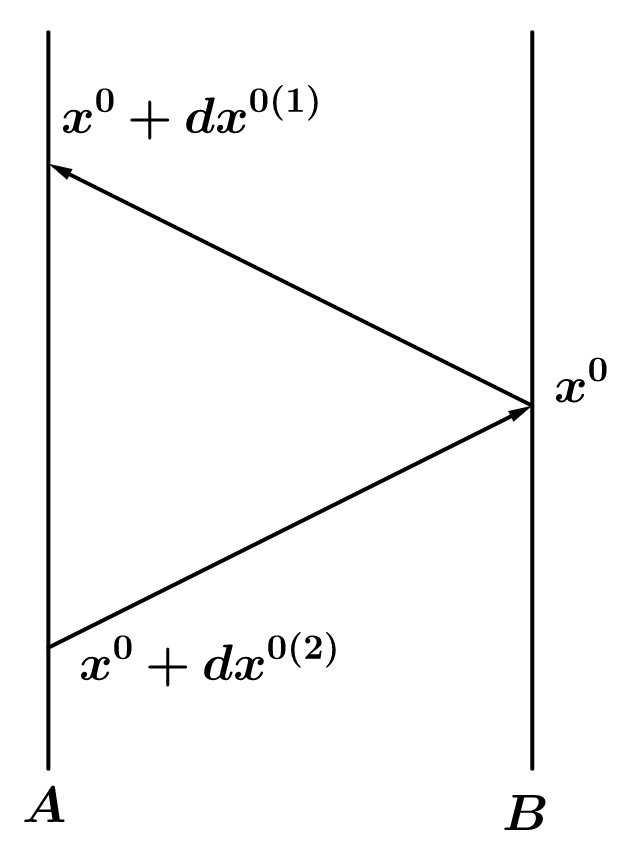
\includegraphics[width=5cm]{Imagenes/Fig17}
\caption[Medición de distancias en sistemas de coordenadas no inerciales.]{Representación esquemática del método de medición de distancias.}
\end{figure}
\begin{eqnarray}
\nonumber ds^{2}=&0&=g_{00}(dx^{0})^{2}+2g_{0i}dx^{0}dx^{i}+g_{ij}dx^{i}dx^{j}\\
\nonumber \Rightarrow dx^{o}&=&\left[-\frac{g_{oi}}{g_{00}}\pm\frac{\sqrt{g_{0i}g_{ok}+g_{00}g_{ik}}dx^{i}dx^{k}}{g_{00}}\right]\\
\Rightarrow dx^{0(2)}&=&\left[-\frac{g_{oi}}{g_{00}}+\frac{\sqrt{g_{0i}g_{ok}+g_{00}g_{ik}}dx^{i}dx^{k}}{g_{00}}\right]\\
\Rightarrow dx^{0(1)}&=&\left[-\frac{g_{oi}}{g_{00}}-\frac{\sqrt{g_{0i}g_{ok}+g_{00}g_{ik}}dx^{i}dx^{k}}{g_{00}}\right],
\end{eqnarray} 
ahora como $\triangle x^0=x^0+dx^{0(1)}-x^0-dx^{0(2)}$ tenemos:
\begin{equation}
\triangle x^0= -2\frac{\sqrt{g_{0i}g_{ok}+g_{00}g_{ik}}dx^{i}dx^{k}}{g_{00}}.
\end{equation}
Por otro lado:
\begin{equation}
dl=\frac{c}{2}\triangle\tau\ \text{y}\ \triangle\tau=\sqrt{-g_{00}}\triangle x^{0}\Rightarrow dl^{2}=\frac{c^{2}}{4}(-g_{00})(\triangle x^{0})^{2}=c^{2}\left(g_{ik}-\frac{g_{oi}g_{ok}}{g_{oo}}\right)dx^{i}dx^{k},
\end{equation}
con este resultado es posible analizar la estructura geométrica del espacio, para un disco que \textbf{no rota} tenemos que $\oint dl=2\pi r$, sin embargo en el caso que estamos estudiando la ecuación (3.158) nos lleva a:
\begin{eqnarray}
\nonumber dl^{2}&=&c^{2}\left(g_{22}-\frac{g_{o2}g_{o2}}{g_{oo}}\right)d\phi^{2},\ \text{para}\ \omega\ll 1\\
\nonumber &=& \left(r^{2}\frac{\frac{\omega^{2}r^{4}}{c^{2}}}{1-\frac{\omega^{2}r^{2}}{c^{2}}}\right)d\phi^{2}\approx \left(r^{2}+\frac{\omega^{2}r^{4}}{c^{2}}\left(1+\frac{\omega^{2}r^{2}}{c^{2}}\right)\right)d\phi^{2}\\
\nonumber &=& \approx r^{2}\left(1+\frac{\omega^{2}r^{2}}{c^{2}}\right)d\phi^{2}\\
\nonumber \Rightarrow dl &\approx &r \left(1+\frac{\omega^{2}r^{2}}{2c^{2}}\right)\\
\Rightarrow\oint dl&=& 2\pi r\left(1+\frac{\omega^{2}r^{2}}{2c^{2}}\right)>2\pi r,
\end{eqnarray}
el espacio es curvo!
\\
\\
Por último estudiemos el problema de la sincronización de relojes,observando la figura 3.1, un evento que es simultáneo en tiempo $x^0$ para $A$ sucede en $B$ justo en la mitad de los enventos de enviar y recibir la luz, es decir en $x^{0}+\frac{dx^{0(1)}+dx^{0(2)}}{2}=x^{0}-\frac{g_{oi}}{g_{00}}dx^{i}\equiv x^{0}+\triangle x^{0}$. En un sistema de referencia \textbf{sin rotación} $g_{oi}=0$ por tanto la sincronización es posible, sin embargo en nuestro caso $g_{0i}\neq 0\Rightarrow \triangle x^0\neq 0$, es por esto que al intentar sincronizar un reloj en una trayectoria cerrada vamos a fracasar debido a que al retornar al punto de partida el reloj 	va a haber acumulado un retraso $\triangle x^{0}=-\oint\frac{g_{oi}}{g_{oo}}dx^{i}$. Las consecuencias experimentales de este fenómeno fueron medidas por primera vez por Georges Sagnac, razón por la cual se conoce a este fenómeno como    \textbf{efecto Sagnac}.
\begin{figure}[h!]
\centering
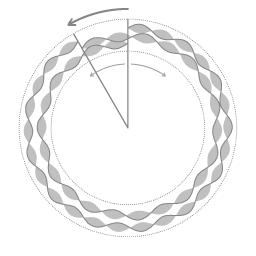
\includegraphics[width=7cm]{Imagenes/Fig18}
\caption[Representación esquemática del efecto Sagnac.]{Representación esquemática del efecto Sagnac, la interferencia se produce debido a la diferencia de camino óptico entre los haz.}
\end{figure}
\\
\\
El efecto Sagnac consiste en el corrimiento de las líneas del patrón de interferencia de dos haz de luz que viajan en direcciones opuestas en un interferómetro rotante, en la figura 3.2 se muestra un esquema del efecto. Calculemos el corrimiento, sabemos que:
\begin{equation}
\triangle t=\frac{1}{c}\triangle x^{0}=\frac{1}{c}\oint\frac{\frac{\omega r^{2}}{c}}{1-\frac{\omega^{2}r^{2}}{c^{2}}}d\phi\approx\frac{\omega}{c^{2}}\oint r^{2}d\phi=\frac{\omega2\pi r^{2}}{c^{2}},
\end{equation}
la discrepancia en tiempo propio para $\omega \ll 1$ es $\triangle \tau =\sqrt{-g_{00}}\triangle t\approx \triangle t$, con esto podemos calcular la longitud de camino óptico:
\begin{equation}
l+\triangle l=2\pi r+c\triangle \tau =L+\frac{2\omega \pi r^2}{c},
\end{equation}  
para el rayo que va en la dirección opuesta:
\begin{equation}
l-\triangle l=L-\frac{2\omega \pi r^2}{c}.
\end{equation}
Por tanto la diferencia de camino óptico es $\frac{4\omega \pi r^2}{c}$, lo que corresponde a un corrimiento:
\begin{equation}
\triangle N= \frac{4\pi r^2\omega}{c\lambda}.
\end{equation}
En el experimento realizado por Sagnac $\omega=14\text{rad/s},\ \pi r^2=0.0863 m^2\ \text{y}\ \lambda=0.436\times10^{-6}m$, al insertar estos datos en (3.163) obtenemos:
\begin{equation}
\triangle N=0.036\ ,
\end{equation}
valor que concuerda con el experimento.
\subsection{El propagador.}
En esta última sección vamos a derivar el propagador para una partícula que se mueve en una trayectoria circular en un espacio-tiempo rotante, como ya hemos visto, en este tipo de sistemas de coordenadas aparecen efectos nuevos, como el efecto Sagnac. Esto último debido a que son sistemas de coordenadas no inerciales, es por esta razón que resulta interesante estudiar este problema desde un punto de vista cuántico.
\\
\\
Para un espacio-tiempo (1+2) dimensional, rotante (con velocidad angular $\omega$), la métrica esta dada por:
\begin{equation}
g_{\mu\nu}=\left(\begin{array}{ccc}
(1-r^{2}\omega^{2}) & 0 & -r^{2}\omega\\
0 & -1 & 0\\
-r^{2}\omega & 0 & -r^{2}
\end{array}\right),
\end{equation}
notemos que hemos cambiado la signatura de la mética a $(-,+,+)$ y de ahora en adelante usaremos unidades naturales $(\hbar=c=G=1)$. Si calculamos el determinante de la ecuación (3.165) obtenemos:
\begin{equation}
\det g_{\mu\nu}=r^{2}\Rightarrow g=\sqrt{\det g_{\mu\nu}}=r,
\end{equation}
este es el mismo resultado que obtendriamos para el caso del espacio de Minkowski en coordenadas polares, por tanto, el espacio-tiempo sigue siendo plano. Una partícula relativista de masa $\mu$, espín cero y que se mueve en un espacio-tiempo curvo obedece la ecuación de Klein-Gordon en espacio curvo:
\begin{equation}
\left(\square-\frac{\mathcal{R}}{8}-\mu^{2}\right)\psi=0\ ;\ \square=g^{\mu\nu}\nabla_{\mu}\nabla_{\nu},
\end{equation} 
donde $\mathcal{R}$ es el escalar de Ricci. El propagador para esta partícula es:
\begin{equation}
K(t^{'},t^{''},r^{'},r^{''},\theta^{'}.\theta^{''})=\int\exp(iS)\mathcal{D}[x],
\end{equation}
donde
\begin{equation}
S=\int_{0}^{\Lambda}\left[\frac{1}{2}g_{\mu\nu}\dot{x}^{\mu}\dot{x}^{\nu}-k^{2}\right]d\lambda\ ;\ k^{2}=\frac{1}{2}\left[-\frac{1}{24}\mathcal{R}+\mu^{2}\right].	
\end{equation}
Sabemos de las secciones anteriores que el término proporcional al escalar de Ricci en la ecuación (3.169) viene del hecho de llevar a cabo el cálculo de la integral de trayectoria en espacio-tiempo curvo, sin embargo, como consecuencia directa de la ecuación (3.166) (el espacio-tiempo es plano), entonces $\mathcal{R}=0$. Tomando en cuenta todo lo anterior:
\begin{equation}
S=\int_{0}^{\Lambda}\left[-\frac{1}{2}\dot{t}^{2}(1-\omega^{2}r^{2})+\frac{\dot{r}^{2}}{2}+\frac{r^{2}\dot{\theta}^{2}}{2}+r^{2}\omega\dot{\theta}\dot{t}-\frac{\mu^{2}}{2}\right]d\lambda.
\end{equation} 
En la expresión anterior hemos usado la notación $\dot{x}\equiv\frac{dx}{d\lambda}$, si escribimos el propagador (3.168) en forma discretizada:
\begin{equation}
K(t^{'},t^{''},r^{'},r^{''},\theta^{'}.\theta^{''})=\lim_{N\to\infty}\int\prod_{j=1}^{N}\exp(iS_{j})\mathcal{D}[x],
\end{equation}
donde:
\begin{equation}
\mathcal{D}[x]=\lim_{N\to\infty}\prod_{j=1}^{N}\left(\frac{1}{2\pi i\epsilon_{j}}\right)^{\frac{3}{2}}\prod_{j=1}^{N-1}g_{j}^{\frac{1}{2}}dt_{j}dr_{j}d\theta_{j}=\lim_{N\to\infty}\prod_{j=1}^{N}\left(\frac{1}{2\pi i\epsilon_{j}}\right)^{\frac{3}{2}}\prod_{j=1}^{N-1}r_{j}dt_{j}dr_{j}d\theta_{j},
\end{equation}
y
\begin{equation}
S_{j}=-\frac{1}{2}(1-\omega^{2}r_{j}^{2})\frac{(\triangle t_{j})^{2}}{\epsilon_{j}}+\frac{(\triangle r_{j})^{2}}{2\epsilon_{j}}+r_{j}^{2}\frac{(\triangle\theta_{j})^{2}}{2\epsilon_{j}}+r_{j}^{2}\omega\frac{\triangle\theta_{j}\triangle t_{j}}{\epsilon_{j}}-\frac{\mu^{2}\epsilon_{j}}{2}.
\end{equation}
Podemos fijar la variable radial a un valor $r=R$, mediante la siguiente relación:
\begin{equation}
\left(\frac{1}{2\pi i\epsilon_{j}}\right)^{\frac{1}{2}}\exp\left(\frac{i(\triangle r_{j})^{2}}{2\epsilon_{j}}\right)=\delta(r_{j}-r_{j-1}),
\end{equation}
por tanto el propagador queda:
\begin{equation}
K(t^{'},t^{''},\theta^{'}.\theta^{''})=\exp\left(-\frac{i\mu^{2}\Lambda}{2}\right)\lim_{N\to\infty}\int\prod_{j=1}^{N}\exp(iS_{j}(t,\theta))\prod_{j=1}^{N}\left(\frac{1}{2\pi i\epsilon_{j}}\right)\prod_{j=1}^{N-1}Rdt_{j}d\theta_{j},
\end{equation}
con
\begin{equation}
S_{j}(t,\theta)=-\frac{1}{2}(1-\omega^{2}R^{2})\frac{(\triangle t_{j})^{2}}{\epsilon_{j}}+R^{2}\frac{(\triangle\theta_{j})^{2}}{2\epsilon_{j}}+R^{2}\omega\frac{\triangle\theta_{j}\triangle t_{j}}{\epsilon_{j}}.
\end{equation}
Si introducimos la variable temporal adimensional $\triangle t_j\omega =\triangle \tau_j$, obtenemos:
\begin{equation}
S_{j}(\tau,\theta)=-\frac{1}{2\epsilon_{j}}\left(\frac{1}{\omega^{2}}-R^{2}\right)(\triangle\tau_{j})^{2}+R^{2}\frac{(\triangle\theta_{j})^{2}}{2\epsilon_{j}}+R^{2}\frac{\triangle\theta_{j}\triangle\tau_{j}}{\epsilon_{j}},
\end{equation}
y el propagador queda escrito como:
\begin{equation}
K(\tau^{'},\tau^{''},\theta^{'},\theta^{''})=\exp\left(-\frac{i\mu^{2}\Lambda}{2}\right)\lim_{N\to\infty}\int\prod_{j=1}^{N}\exp(iS_{j}(\tau,\theta))\prod_{j=1}^{N}\left(\frac{1}{2\pi i\epsilon_{j}}\right)\prod_{j=1}^{N-1}\frac{R}{\omega}d\tau_{j}d\theta_{j}.
\end{equation}
Ahora con el fin de eliminar el término proporcional a $\triangle \theta_j\triangle \tau_j$, es decir separar de nuevo las coordenadas, hagamos una rotación de las mismas. Si se tiene una forma cuadrática $F=Ax^2+Bxy+Cy^2$, podemos hacer una rotación de tal manera que es posible escribir $F=A^{'}x^{'2}+C^{'}y^{'2}$, para que esto se cumpla debemos tener que $\cot (2\phi)=\frac{A-C}{B}$, en este caso el término $xy$ se anula y tenemos que:
\begin{align}
\nonumber A^{'}&=A\cos^{2}\phi+B\sin\phi\cos\phi+C\sin^{2}\phi\\
B^{'}&=A\sin^{2}\phi-B\sin\phi\cos\phi+C\cos^{2}\phi.
\end{align}
Observando la ecuación (3.177), en nuestro caso:
\begin{equation}
A=-\frac{1}{2\epsilon_{j}}\left(\frac{1}{\omega^{2}}-R^{2}\right),\ B=\frac{R^{2}}{\epsilon_{j}},\ C=\frac{R^{2}}{2\epsilon_{j}},
\end{equation}
así:
\begin{equation}
\cot(2\phi)=-\frac{1}{2R^{2}\omega^{2}}.
\end{equation}
Acudiendo a la Figura 3.3, escribimos las siguientes relaciones:
\begin{figure}[h!]
\centering
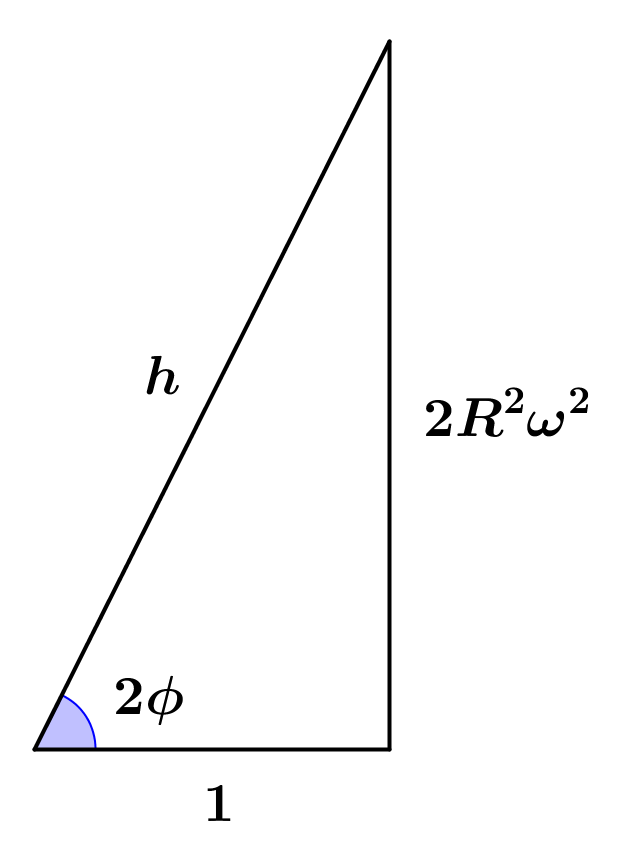
\includegraphics[width=3.8cm]{Imagenes/Fig19}
\caption[Triángulo de funciones trigonométricas.]{Triángulo para la construcción de funciones trigonométricas.}
\end{figure}
\begin{align}
\nonumber h&=\sqrt{1+4R^4\omega^4}\\
\nonumber \cos(2\phi)&=-\frac{1}{h}\\
\nonumber \sin\phi&=\sqrt{\frac{1-\cos2\phi}{2}}=\sqrt{\frac{h+1}{2h}}\\
\nonumber \cos\phi&=\sqrt{\frac{1+\cos2\phi}{2}}=\sqrt{\frac{h-1}{2h}}\\
\sin\phi\cos\phi&=\frac{R^{2}\omega^{2}}{h}.
\end{align}
Combinando las ecuaciones (3.179) y (3.182), obtenemos:
\begin{align}
\nonumber A^{'}&=\frac{1}{2\epsilon_{j}}\left[R^{2}+\frac{1}{2h\omega^{2}}-\frac{1}{2\omega^{2}}+\frac{2R^{4}\omega^{2}}{h}\right]\\
C^{'}&=\frac{1}{2\epsilon_{j}}\left[R^{2}-\frac{1}{2h\omega^{2}}-\frac{1}{2\omega^{2}}-\frac{2R^{4}\omega^{2}}{h}\right],
\end{align}
por tanto:
\begin{equation}
K(\bar{\tau}^{'},\bar{\tau}^{''},\bar{\theta}^{'},\bar{\theta}^{''})=\exp\left(-\frac{i\mu^{2}\Lambda}{2}\right)\lim_{N\to\infty}\int\prod_{j=1}^{N}\exp(iS_{j}(\bar{\tau},\bar{\theta}))\prod_{j=1}^{N}\left(\frac{1}{2\pi i\epsilon_{j}}\right)\prod_{j=1}^{N-1}\frac{R}{\omega}d\bar{\tau}_{j}d\bar{\theta}_{j},
\end{equation}
donde
\begin{equation}
S_{j}(\bar{\tau},\bar{\theta})=A^{'}(\triangle\bar{\tau}_{j})^{2}+C^{'}(\triangle\bar{\theta}_{j})^{2}.
\end{equation}
En estas últimas dos expresiones hemos denotado las coordenadas rotadas como $\bar{\tau},\bar{\theta}$ y debido a que la transformación es una rotación, los diferenciales no se premultiplican por ningún factor debido a que $\det J=1$. Si escribimos:
\begin{equation}
S_{j}(\bar{\tau},\bar{\theta})=\left(\frac{1}{2\epsilon_{j}}\right)\alpha(\triangle\bar{\tau}_{j})^{2}+\left(\frac{1}{2\epsilon_{j}}\right)\beta(\triangle\bar{\theta}_{j})^{2},
\end{equation}
con
\begin{equation}
\alpha=\left[R^{2}+\frac{1}{2h\omega^{2}}-\frac{1}{2\omega^{2}}+\frac{2R^{4}\omega^{2}}{h}\right],\ \beta=\left[R^{2}-\frac{1}{2h\omega^{2}}-\frac{1}{2\omega^{2}}-\frac{2R^{4}\omega^{2}}{h}\right].
\end{equation}
Si ahora $T_j=\frac{1}{\omega}\bar{\tau}_j$ y $R\bar{\theta}_j=\Theta_j$, tenemos que la ecuación (3.184) se transforma en:
\begin{equation}
K(T^{'},T^{''},\Theta^{'},\Theta^{''})=\exp\left(-\frac{i\mu^{2}\Lambda}{2}\right)\lim_{N\to\infty}\int\prod_{j=1}^{N}\exp(iS_{j}(T,\Theta))\prod_{j=1}^{N}\left(\frac{1}{2\pi i\epsilon_{j}}\right)\prod_{j=1}^{N-1}dT_{j}d\Theta_{j},
\end{equation}
donde:
\begin{eqnarray}
\nonumber &S_{j}(T,\Theta)=\left(\frac{1}{2\epsilon_{j}}\right)\alpha^{'}(\triangle T_{j})^{2}+\left(\frac{1}{2\epsilon_{j}}\right)\beta^{'}(\triangle\Theta_{j})^{2}&\\
&\alpha^{'}=\left[R^{2}\omega^{2}+\frac{1}{2h}-\frac{1}{2}+\frac{2R^{4}\omega^{4}}{h}\right],\ \beta^{'}=\left[1-\frac{1}{2hR^{2}\omega^{2}}-\frac{1}{2R^{2}\omega^{2}}-\frac{2R^{2}\omega^{2}}{h}\right]&.
\end{eqnarray}
Después de toda la manipulación que hemos hecho a la expresión (3.175), hasta llevarla a (3.188), por fin hemos logrado obtener una forma funcional como la que ya hemos integrado en la sección $\mathsection$2.1.1, en general el resultado que descubrimos en esa sección se puede escribir como:
\begin{equation}
\lim_{N\to\infty}\int\prod_{j=1}^{N}\exp\left(\frac{ia(\triangle x_{j})^{2}}{2\epsilon_{j}}\right)\prod_{j=1}^{N}\left(\frac{1}{2\pi i\epsilon_{j}}\right)^{\frac{1}{2}}\prod_{j=1}^{N-1}dx_{j}=\left(\frac{A}{2\pi i\Lambda}\right)^{\frac{1}{2}}\exp\left(\frac{iA}{2\Lambda}(x_{N}-x_{0})^{2}\right),
\end{equation}
usando este resultado en (3.188) obtenemos:
\begin{equation}
K(T^{'},T^{''},\Theta^{'},\Theta^{''})=\exp\left(-\frac{i\mu^{2}\Lambda}{2}\right)\left(\frac{\alpha^{'}\beta^{'}}{(2\pi i\Lambda)^{2}}\right)^{\frac{1}{2}}\exp\left(\frac{i\alpha^{'}}{2\Lambda}(T_{N}-T_{0})^{2}\right)\exp\left(\frac{i\beta^{'}}{2\Lambda}(\Theta{}_{N}-\Theta_{0})^{2}\right).
\end{equation}
Para finalizar debemos devolver todas las transformaciones que hemos realizado, primero $T\to\frac{1}{\omega}\bar{\tau}$ y $\Theta\to R\bar{\theta}$, por tanto:
\begin{equation}
K(\bar{\tau}^{'},\bar{\tau}^{''},\bar{\theta}^{'},\bar{\theta}^{''})=\exp\left(-\frac{i\mu^{2}\Lambda}{2}\right)\left(\frac{\alpha\beta\omega^2}{(2\pi i\Lambda)^{2}R^2}\right)^{\frac{1}{2}}\exp\left(\frac{i\alpha}{2\Lambda}(\bar{\tau}^{''}-\bar{\tau}^{'})^{2}\right)\exp\left(\frac{i\beta}{2\Lambda}(\bar{\theta}^{''}-\bar{\theta}^{'})^{2}\right),
\end{equation}
notemos que en la expresión (3.192) ya no usamos $\alpha^{'},\beta^{'}$, sino $\alpha,\beta$. La rotación que realizamos se puede escribir como:
\begin{eqnarray}
\nonumber \bar{\tau}&=\tau\cos\phi+\theta\sin\phi\Rightarrow\bar{\tau}^{2}=\tau^{2}\cos^{2}\phi+\tau\theta2\sin\phi\cos\phi+\theta^{2}\sin^{2}\phi\\
\bar{\theta}&=-\tau\sin\phi+\theta\cos\phi\Rightarrow\bar{\theta}^{2}=\tau^{2}\sin^{2}\phi-\tau\theta2\sin\phi\cos\phi+\theta^{2}\cos^{2}\phi ,
\end{eqnarray} 
así podemos escribir:
\begin{eqnarray}
\nonumber K(\tau^{'},\tau^{''},\theta^{'},\theta^{''})&\propto &\exp\left(\frac{i}{2\Lambda}\left[(\tau^{''}-\tau^{'})^{2}(\alpha\cos^{2}\phi+\beta\sin^{2}\phi)+(\theta^{''}-\theta^{''})^{2}(\alpha\sin^{2}\phi+\beta\cos^{2}\phi)\right]\right)\\
\nonumber &\times & \exp\left(\frac{i}{2\Lambda}\left[(\tau^{''}-\tau^{'})(\theta^{''}-\theta^{''})2\sin\phi\cos\phi(\alpha-\beta)\right]\right)\\
\nonumber &\propto & \exp\left(\frac{i}{2\Lambda}\frac{(\tau^{''}-\tau^{'})^{2}}{2}\left[R^{2}-\frac{1}{2\omega^{2}}-\frac{1}{2\omega^{2}h^{2}}-\frac{2R^{4}\omega^{2}}{h^{2}}\right]\right)\\
\nonumber &\times & \exp\left(\frac{i}{2\Lambda}\frac{(\theta^{''}-\theta^{''})^{2}}{2}\left[R^{2}-\frac{1}{2\omega^{2}}+\frac{1}{2\omega^{2}h^{2}}+\frac{2R^{4}\omega^{2}}{h^{2}}\right]\right)\\
&\times & \exp\left(\frac{i}{2\Lambda}(\tau^{''}-\tau^{'})(\theta^{''}-\theta^{''})\frac{2R^{2}\omega^{2}}{h^{2}}\left[\frac{1}{\omega^{2}}+4R^{4}\omega^{2}\right]\right).
\end{eqnarray}
Finalmente si hacemos la última sustitución, $\tau \to \omega t$:
\begin{eqnarray}
\nonumber K(t^{'},t^{''},\theta^{'},\theta^{''})&=&\exp\left(-\frac{i\mu^{2}\Lambda}{2}\right)\left(\frac{\alpha\beta\omega^2}{(2\pi i\Lambda)^{2}R^2}\right)^{\frac{1}{2}}\exp\left(\frac{i}{2\Lambda}\frac{(t^{''}-t^{'})^{2}}{2}\left[R^{2}\omega^{2}-\frac{1}{2}-\frac{1}{2h^{2}}-\frac{2R^{4}\omega^{4}}{h^{2}}\right]\right)\\
\nonumber &\times & \exp\left(\frac{i}{2\Lambda}\frac{(\theta^{''}-\theta^{''})^{2}}{2}\left[R^{2}-\frac{1}{2\omega^{2}}+\frac{1}{2\omega^{2}h^{2}}+\frac{2R^{4}\omega^{2}}{h^{2}}\right]\right)\\
&\times &\exp\left(\frac{i}{2\Lambda}(t^{''}-t^{'})(\theta^{''}-\theta^{''})\left[\frac{2R^{2}\omega}{h^{2}}+\frac{8R^{6}\omega^{5}}{h^{2}}\right]\right),
\end{eqnarray} 
una forma de realizar una prueba de consistencia al resultado (3.195) es explorar el límite $\omega \to 0$, si tomamos este límite en (3.195) vemos que:
\begin{equation}
K(t^{'},t^{''},\theta^{'},\theta^{''})_{\omega\to0}=\exp\left(-\frac{i\mu^{2}\Lambda}{2}\right)\left(\frac{1}{2\pi\Lambda}\right)\exp\left(\frac{i}{2\Lambda}\left[-\frac{(t^{''}-t^{'})^{2}}{2}+\frac{(\theta^{''}-\theta^{''})^{2}}{2}R^{2}\right]\right).
\end{equation} 
Esto debido a que $\lim_{\omega\to 0}\left(\alpha\beta\frac{\omega^2}{R^2}\right)^{\frac{1}{2}}=i$, vemos que la expresión (3.196) tiene las coordenadas desacopladas y no depende de $\omega$, esto era lo esperado.